\section{Forums}

\subsection{Overview Page}
The forums are accessible from the sidebar of a course page. Each topic group has a dedicated forum.

When first opening the forums, the user would see the forum overview page.

\newpage

\begin{figure}[h!]
    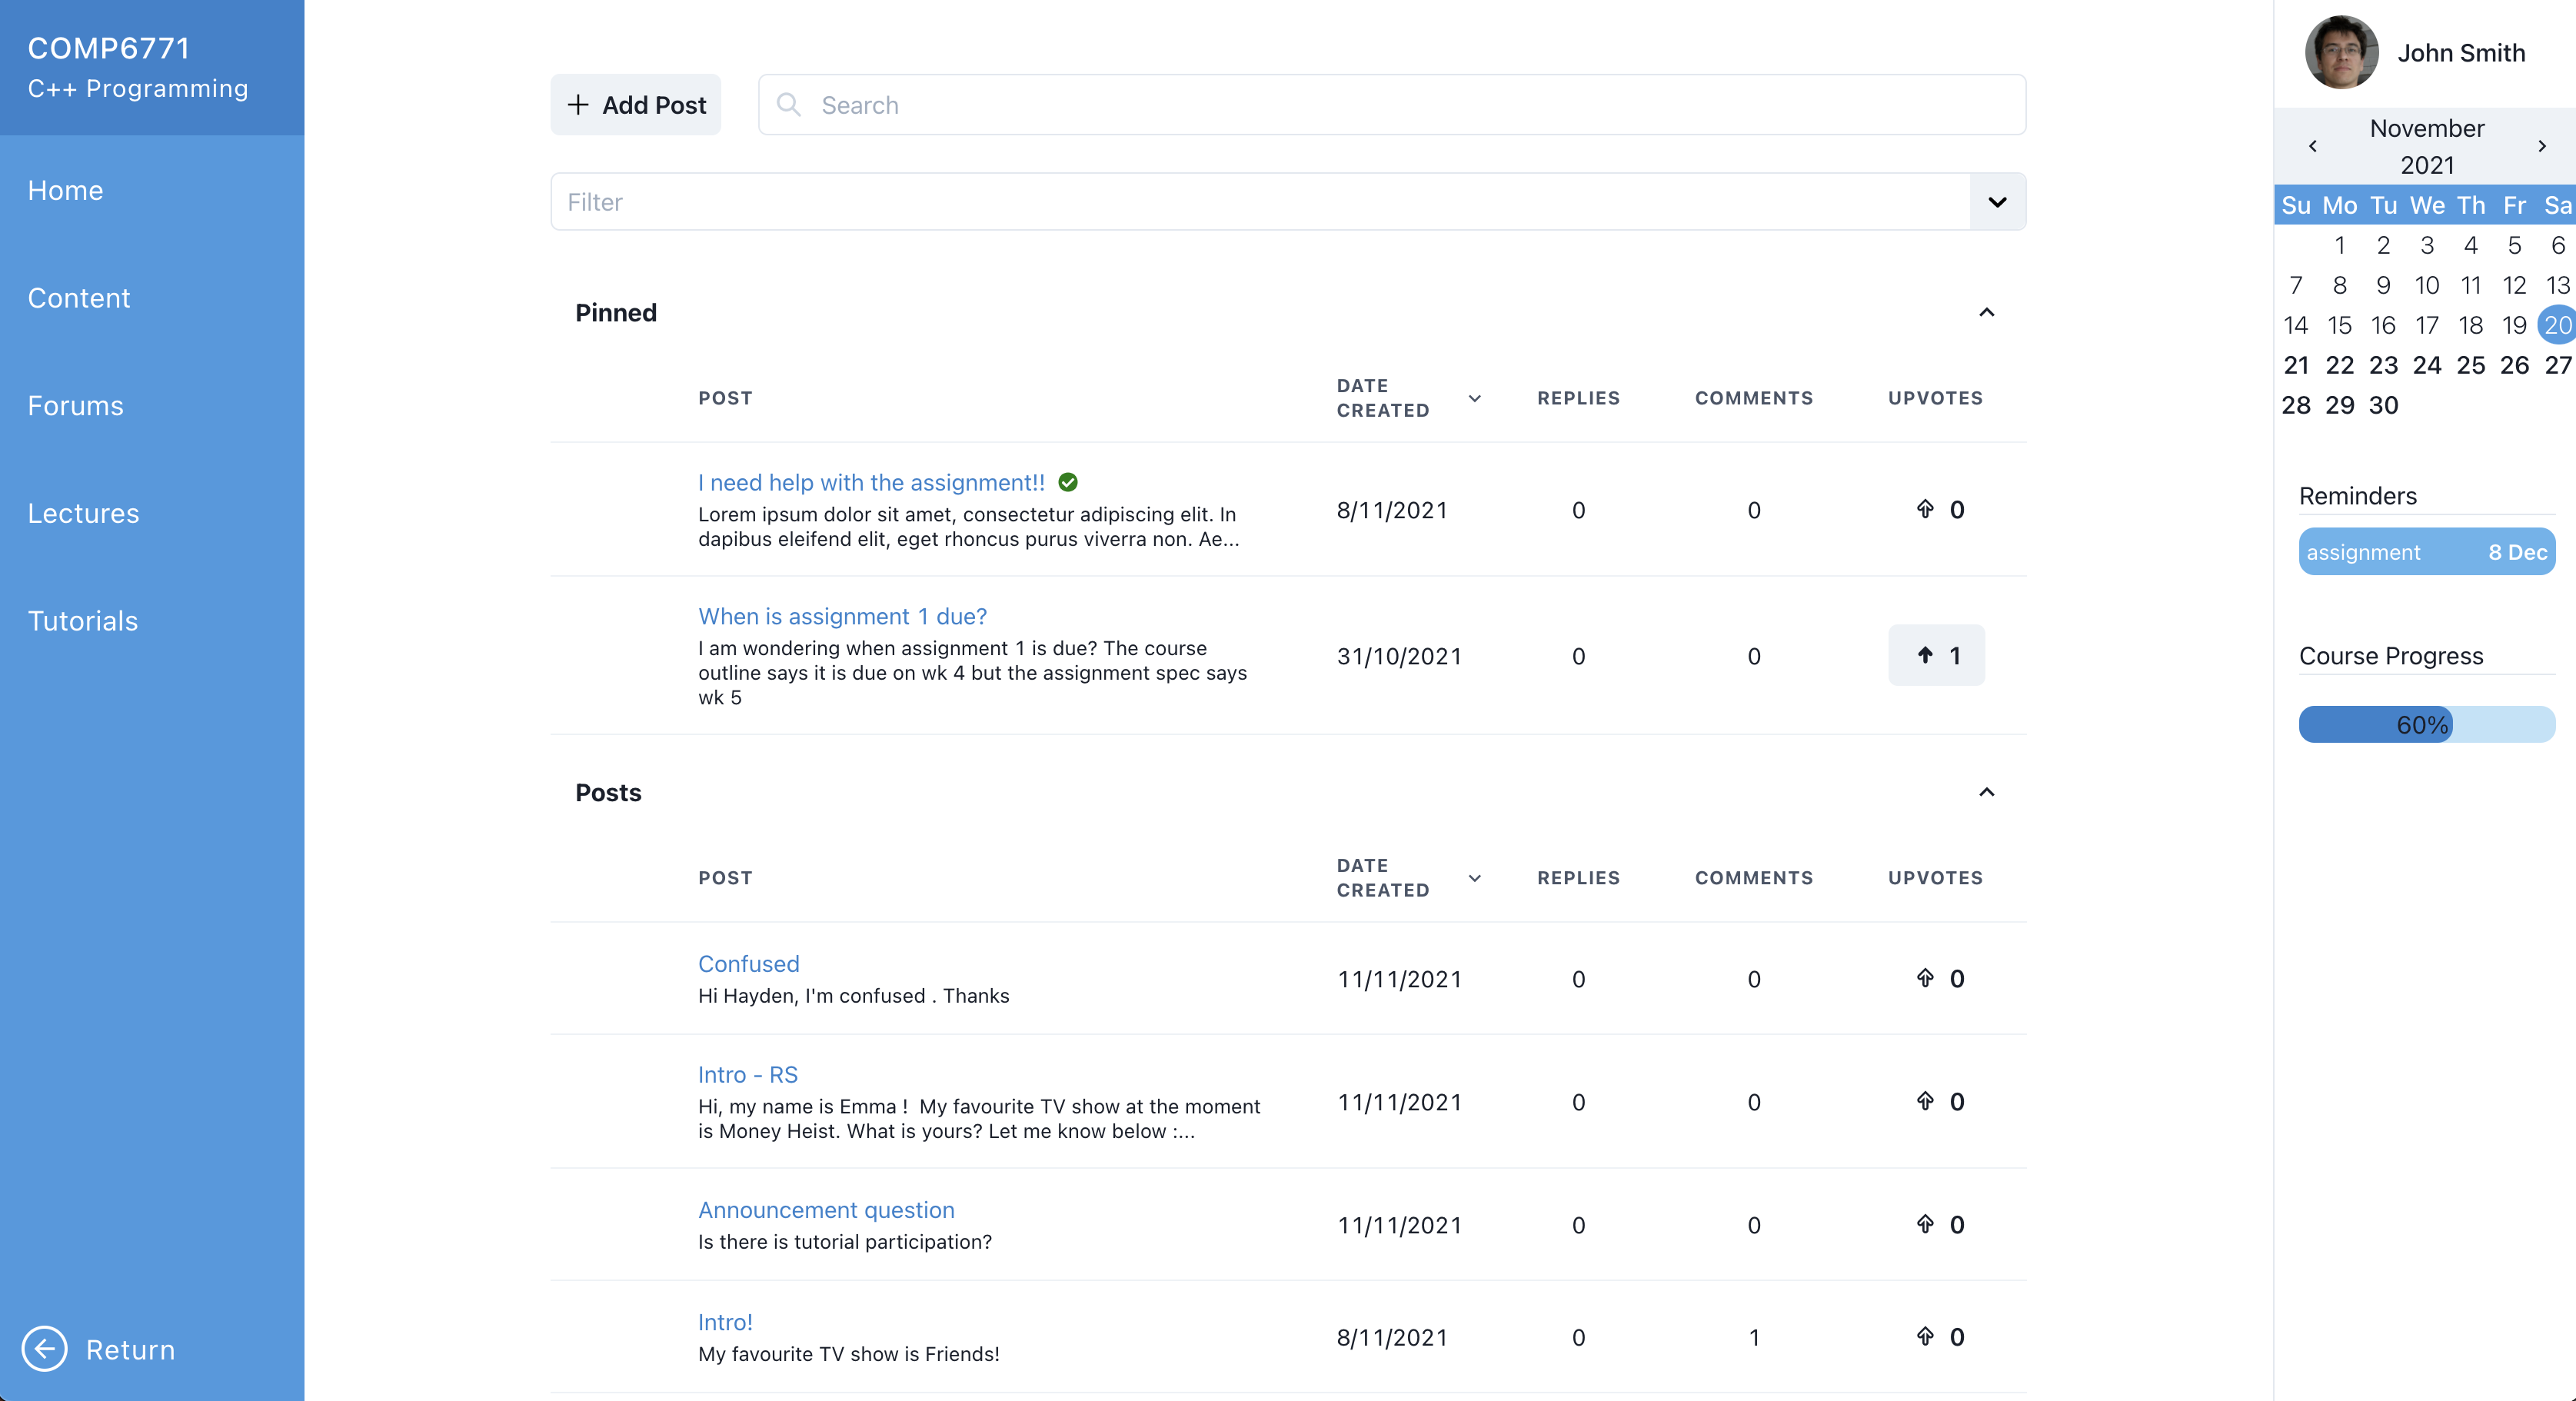
\includegraphics[scale=0.2]{forums-walkthrough-overview-page.png}
    \centering
    \caption{Forum overview page for a student.}
\end{figure}

\subsubsection{Purpose}
Shows users an overview of all the posts that have been posted on the forum page.

\subsubsection{What Was Implemented}
The forum overview page is split into two different tables, the pinned posts and all posts in reverse chronological order.
Within each table, there are columns for the post title and description, date created, number of replies, number of comments, and upvotes.
Posts that are endorsed are shown with a green check mark.
A user can change the post order by clicking the heading of each table. This will toggle the column's order between decreasing and increasing.
At the top of the forum overview page, there is a button to add posts, a search bar and a filter menu.

\subsubsection{How It Was Implemented}
The system uses the course code that is in the url of the site to get the correct forum data from the backend.
When the page loads, two backend calls are made to populate the post tables - one to grab all the posts, and another to grab the pinned posts.
The React library, \texttt{react-table} was used to add the sorting functionality.
It takes a list of column objects that define the heading and contents for the column.

\subsubsection{Considerations}
Instead of having a single post list with the pinned posts marked with a pin icon to highlight that it was different, a separate pinned post table was built.
This is to bring more attention to the pinned posts and make them easier to find.

The post tables were made collapsible to prevent users having to scroll past many pinned posts in order to see the rest.

\subsection{Add Post}
Posts can be added using the call-to-action button on the top left corner of the forum overview page.
Clicking this button will open up the add post modal.

\begin{figure}[h!]
    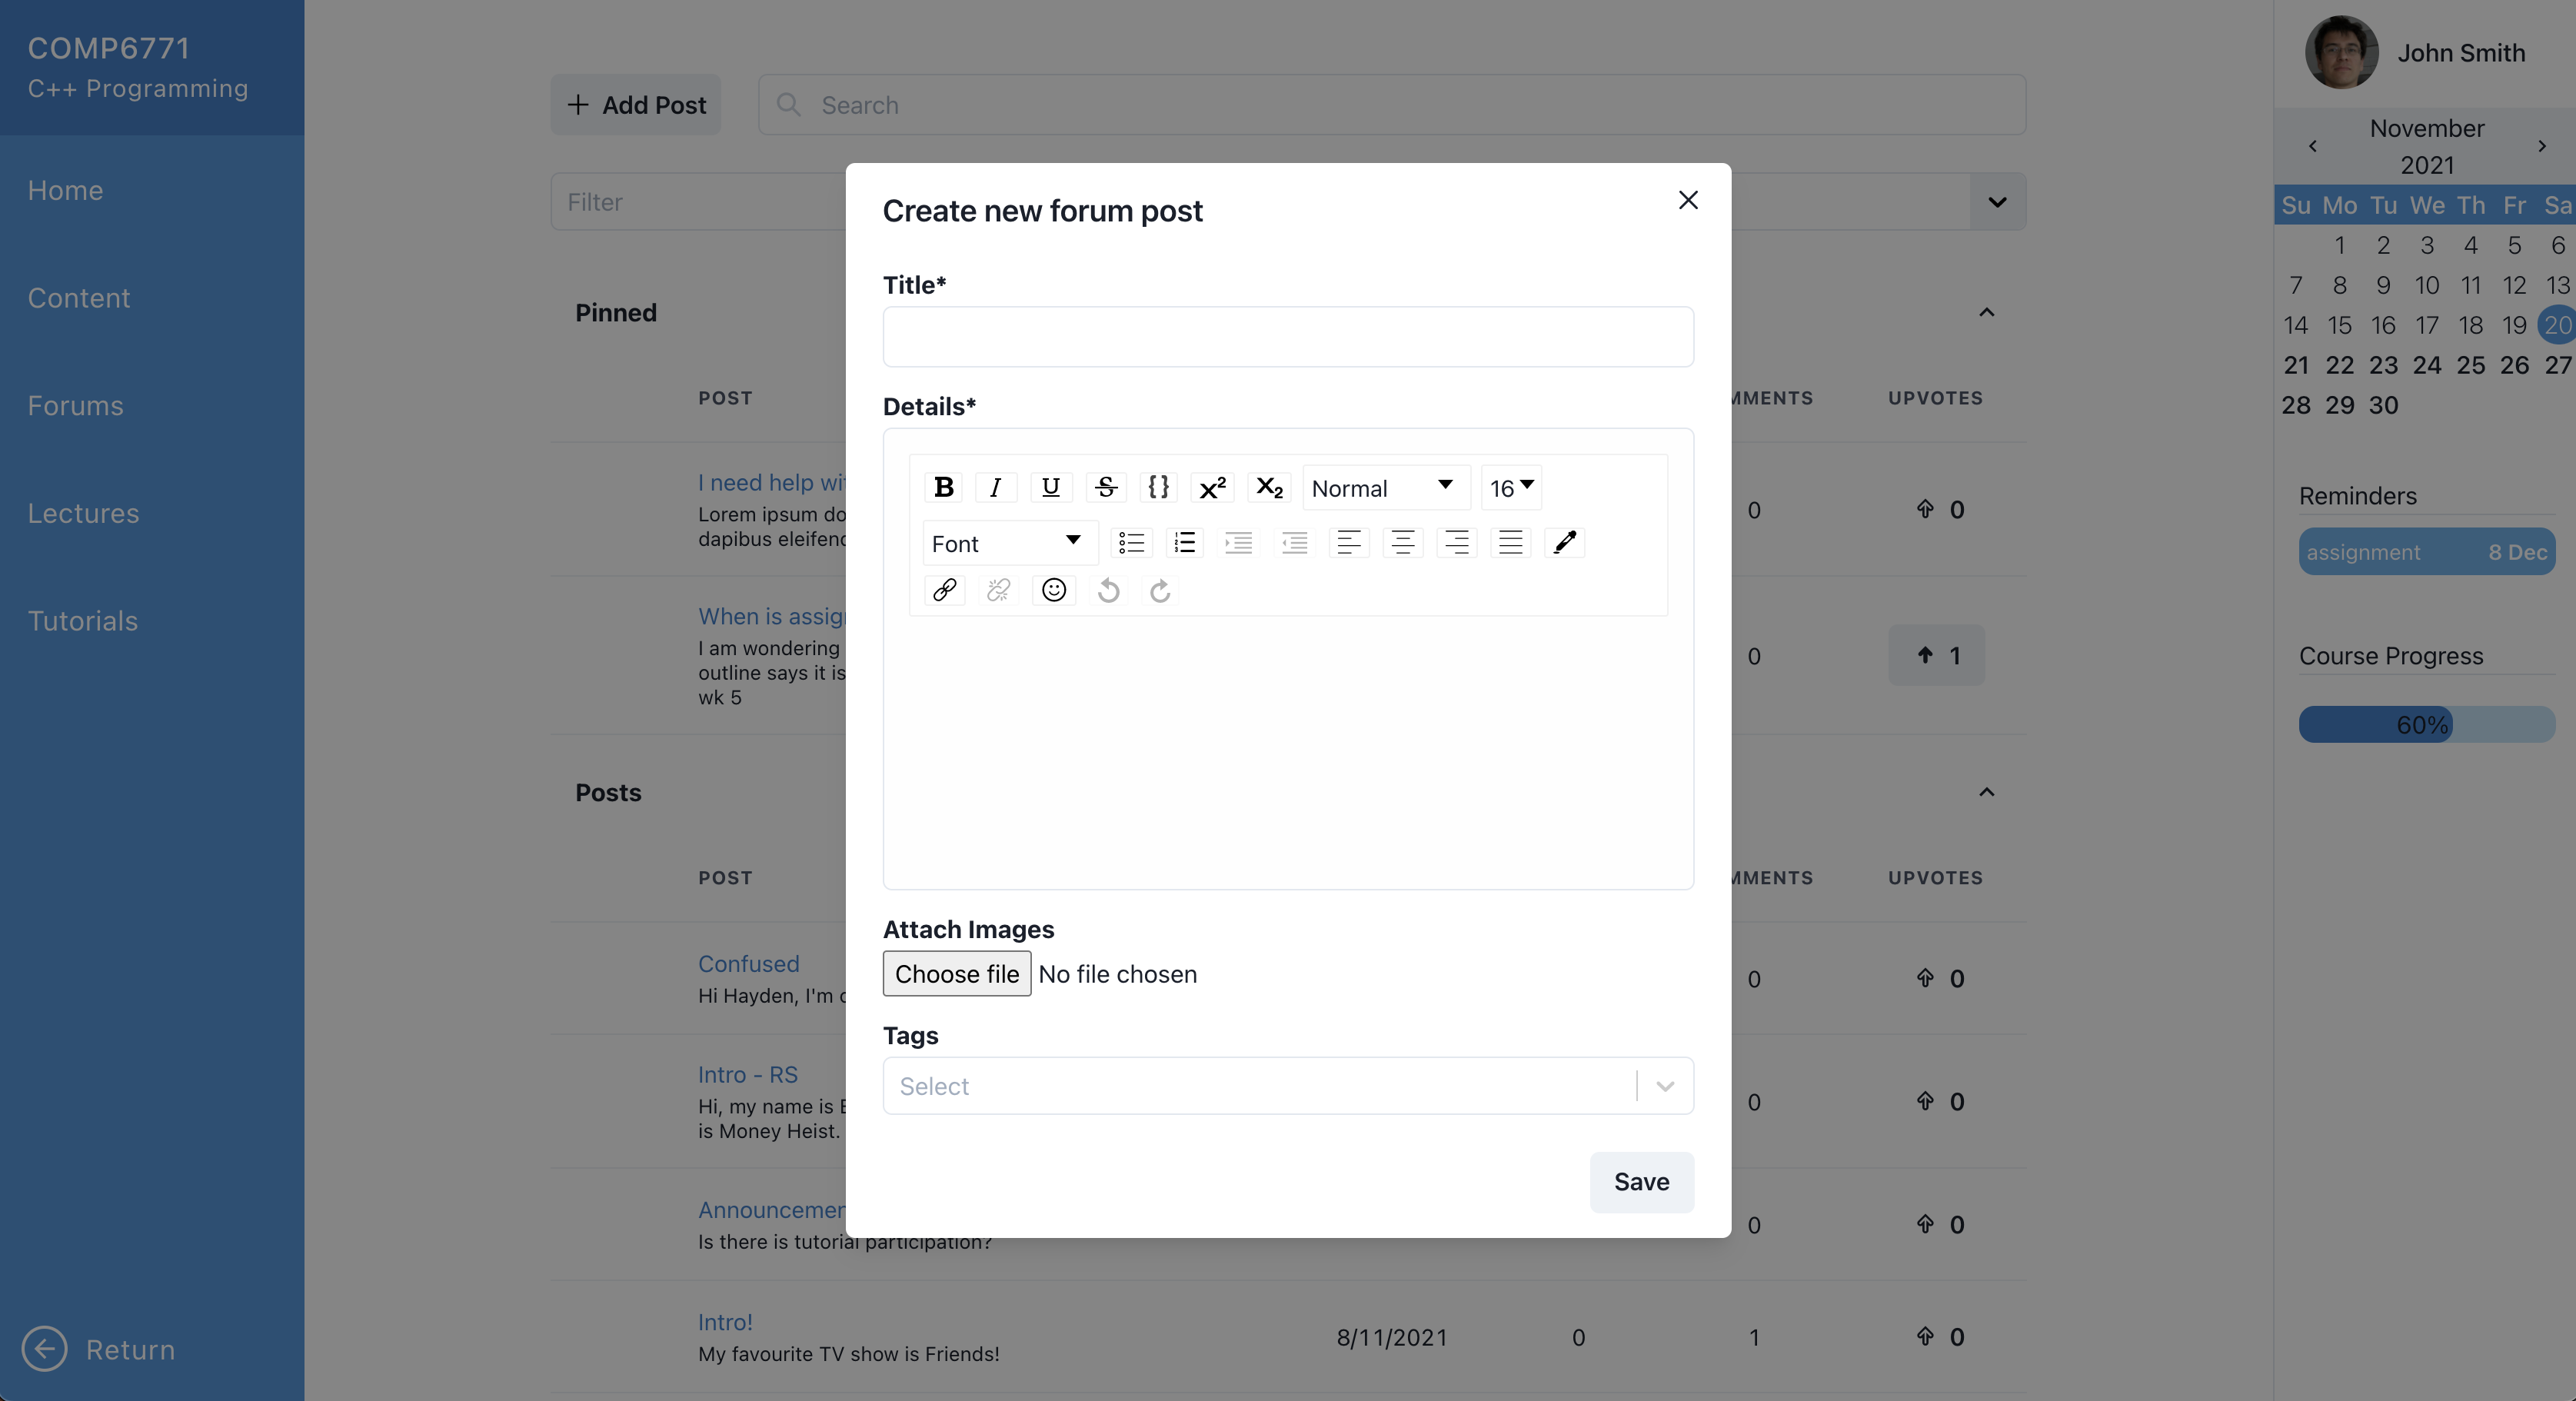
\includegraphics[scale=0.2]{forums-walkthrough-add-post.png}
    \centering
    \caption{Add post modal.}
\end{figure}

\subsubsection{Purpose}
Allows any user to easily add their own forum post to ask a question or make a comment.

\subsubsection{What Was Implemented}
The modal that shows when a user clicks the ``Add Post" button allows the user to input a title and description for their post.
They can also attach an image, as well as select tags that apply to the post. The tags help with categorising and filtering the posts.

\subsubsection{How It Was Implemented}
The modal shown is part of the \texttt{chakra-ui} library.
For the details section, the React package \texttt{react-draft-wysiwyg} was used so that the users had a rich text editor to interact with.
The attachments use Javascript's built-in \texttt{input} element and file handling.
When the modal opens, a backend call is made to pull the tag data for the current course page.
The list of tags are passed into the \texttt{react-select} component as options and the \texttt{isMulti} attribute is set to allow users to select multiple tags for their post.
As the fields for title, details, images and tags are populated, the inputs are stored and sent to the backend when the user clicks ``Save".
Saving the post takes the user directly to the post page.

\subsubsection{Considerations}
A modal is used, instead of navigating users to a new page, to keep the add post flow as simple as possible.

For the rich-text-editor, the \texttt{draft-js} package was originally used because of its various plugins, including allowing users to use markdown syntax when typing
however, the switch to \texttt{react-draft-wysiwyg} was made since it was easier to work with and already had the required formatting options built in by default.
In doing this, the markdown syntax option was lost however, the tradeoff was worth it since \texttt{react-draft-wysiwyg} provides the user with far more formatting options.

Due to time constraints, only images can be attached to a forum post.
Since screenshots are typically used to assist when asking a question on forums, it was decided that it was more useful to at least have the option to attach an image than not having any attachment options at all.

\subsection{Search and Filter}
The search and filter options sit at the top of the forum overview page, making it easily accessible for users.

\newpage

\begin{figure}[h!]
    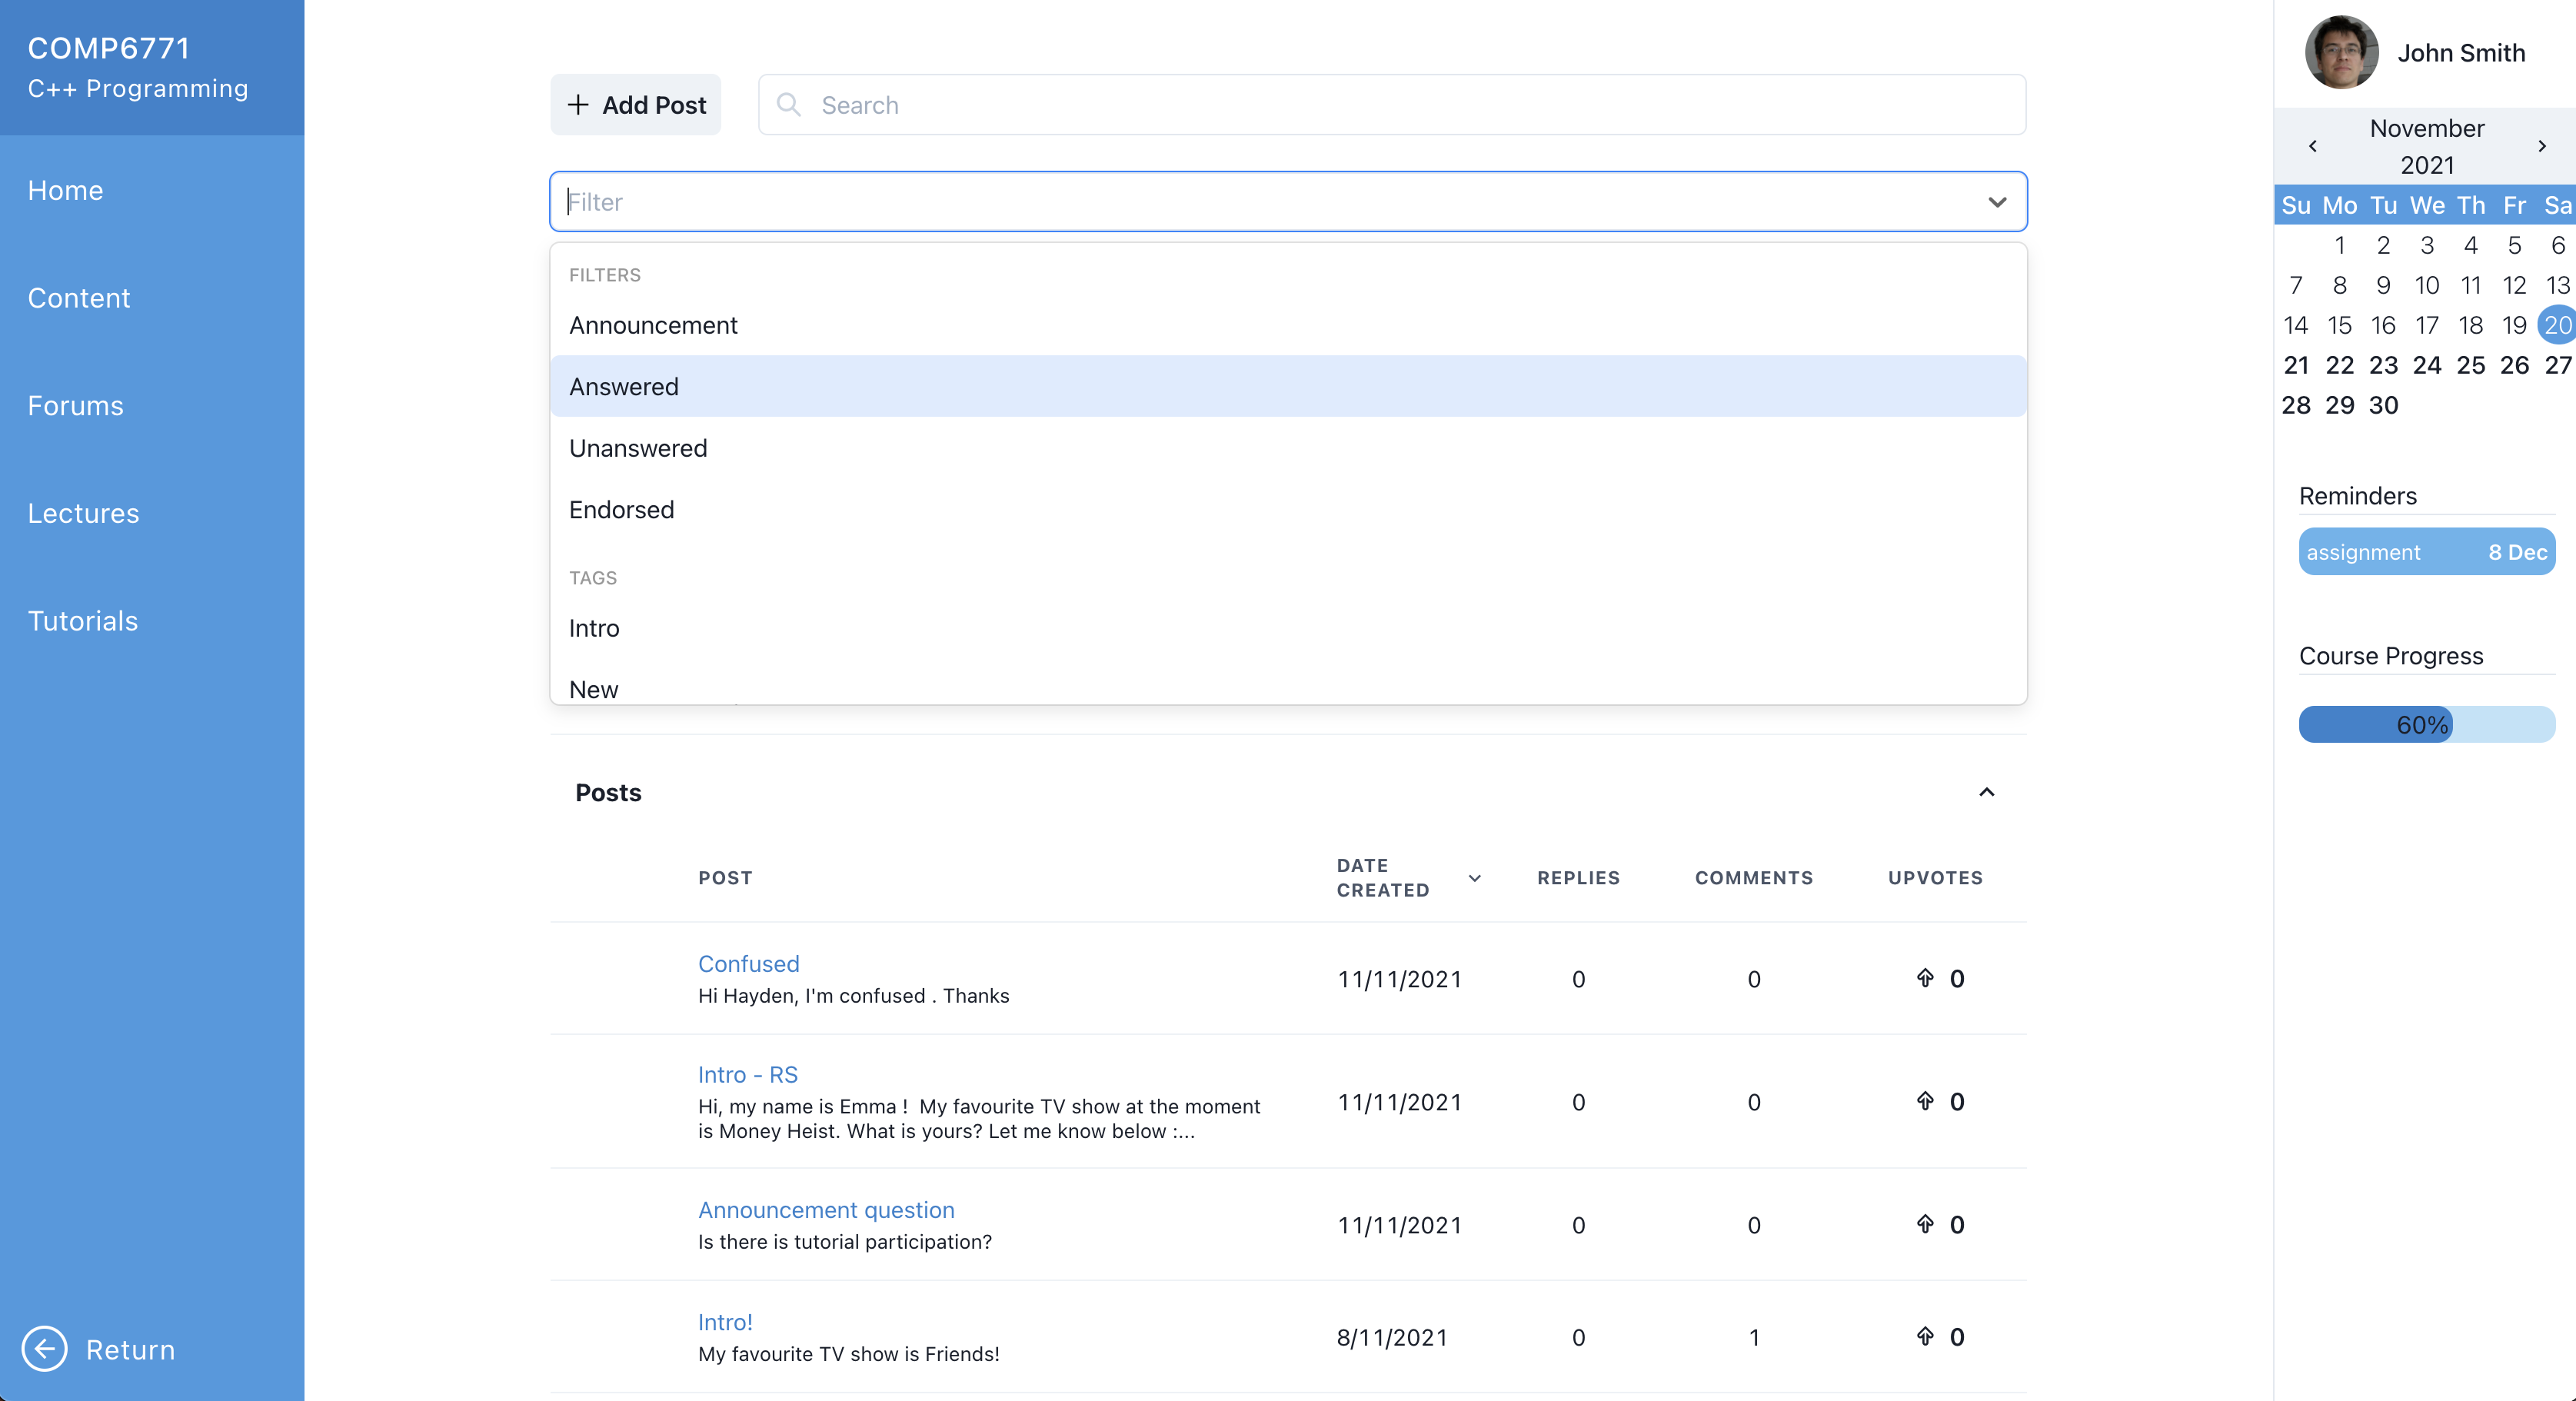
\includegraphics[scale=0.2]{forums-walkthrough-search-filter-sort.png}
    \centering
    \caption{Search bar and filter options}
\end{figure}

\subsubsection{Purpose}
Allows users to easily search for a specific post or filter through posts.

\subsubsection{What Was Implemented}
The search bar is a simple input field that the users can use to search through posts.
The search queries the title and descriptions of each post.
The search results are shown in a table and the ``Pinned" posts table is hidden.

\begin{figure}[h!]
    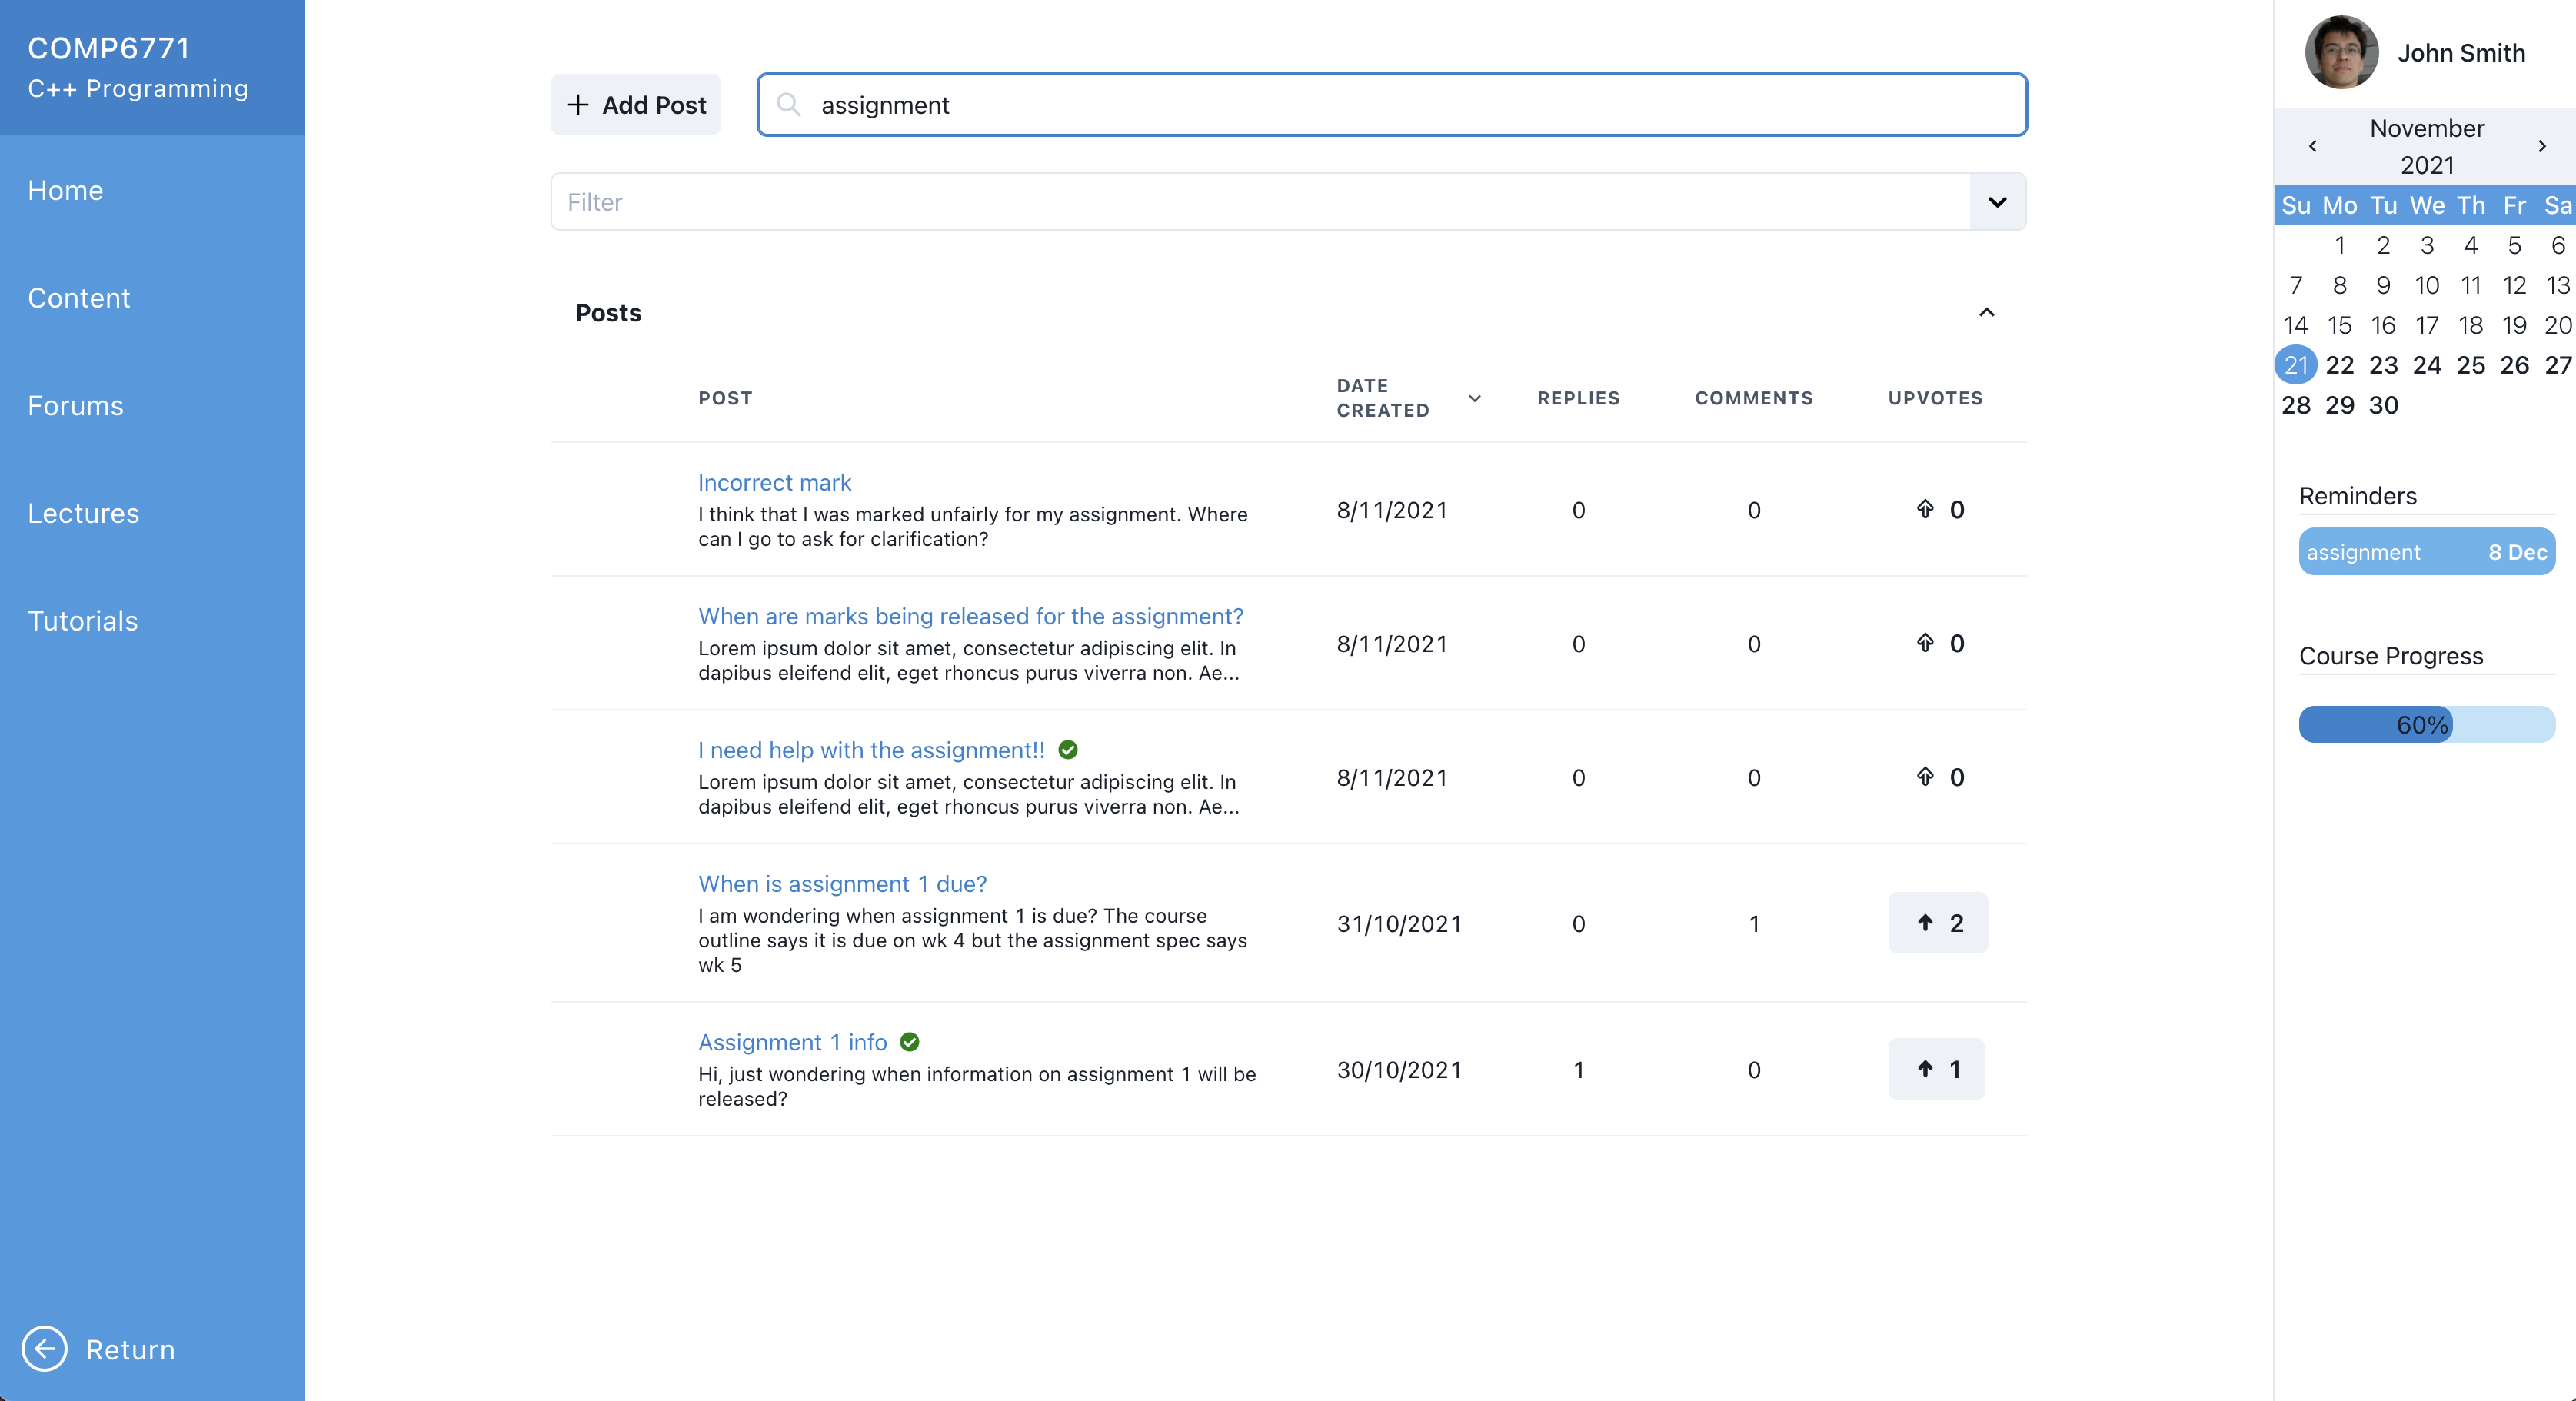
\includegraphics[scale=0.2]{forums-walkthrough-search-results.png}
    \centering
    \caption{Search results when searching for ``assignment"}
\end{figure}

\newpage

Users have two options to filter the posts by, they can either use the tags that have been defined by course staff, or they can filter by the pre-defined filters.
The pre-defined filters consist of posts linked to announcements, answered posts, unanswered posts and endorsed posts.
A user can also use one or more tags when filtering the posts.
A user can either select their filter in the menu or by typing the filter into the filter bar.
Similar to search, the filter results are shown in a table and the ``Pinned" posts table is hidden.

\begin{figure}[h!]
    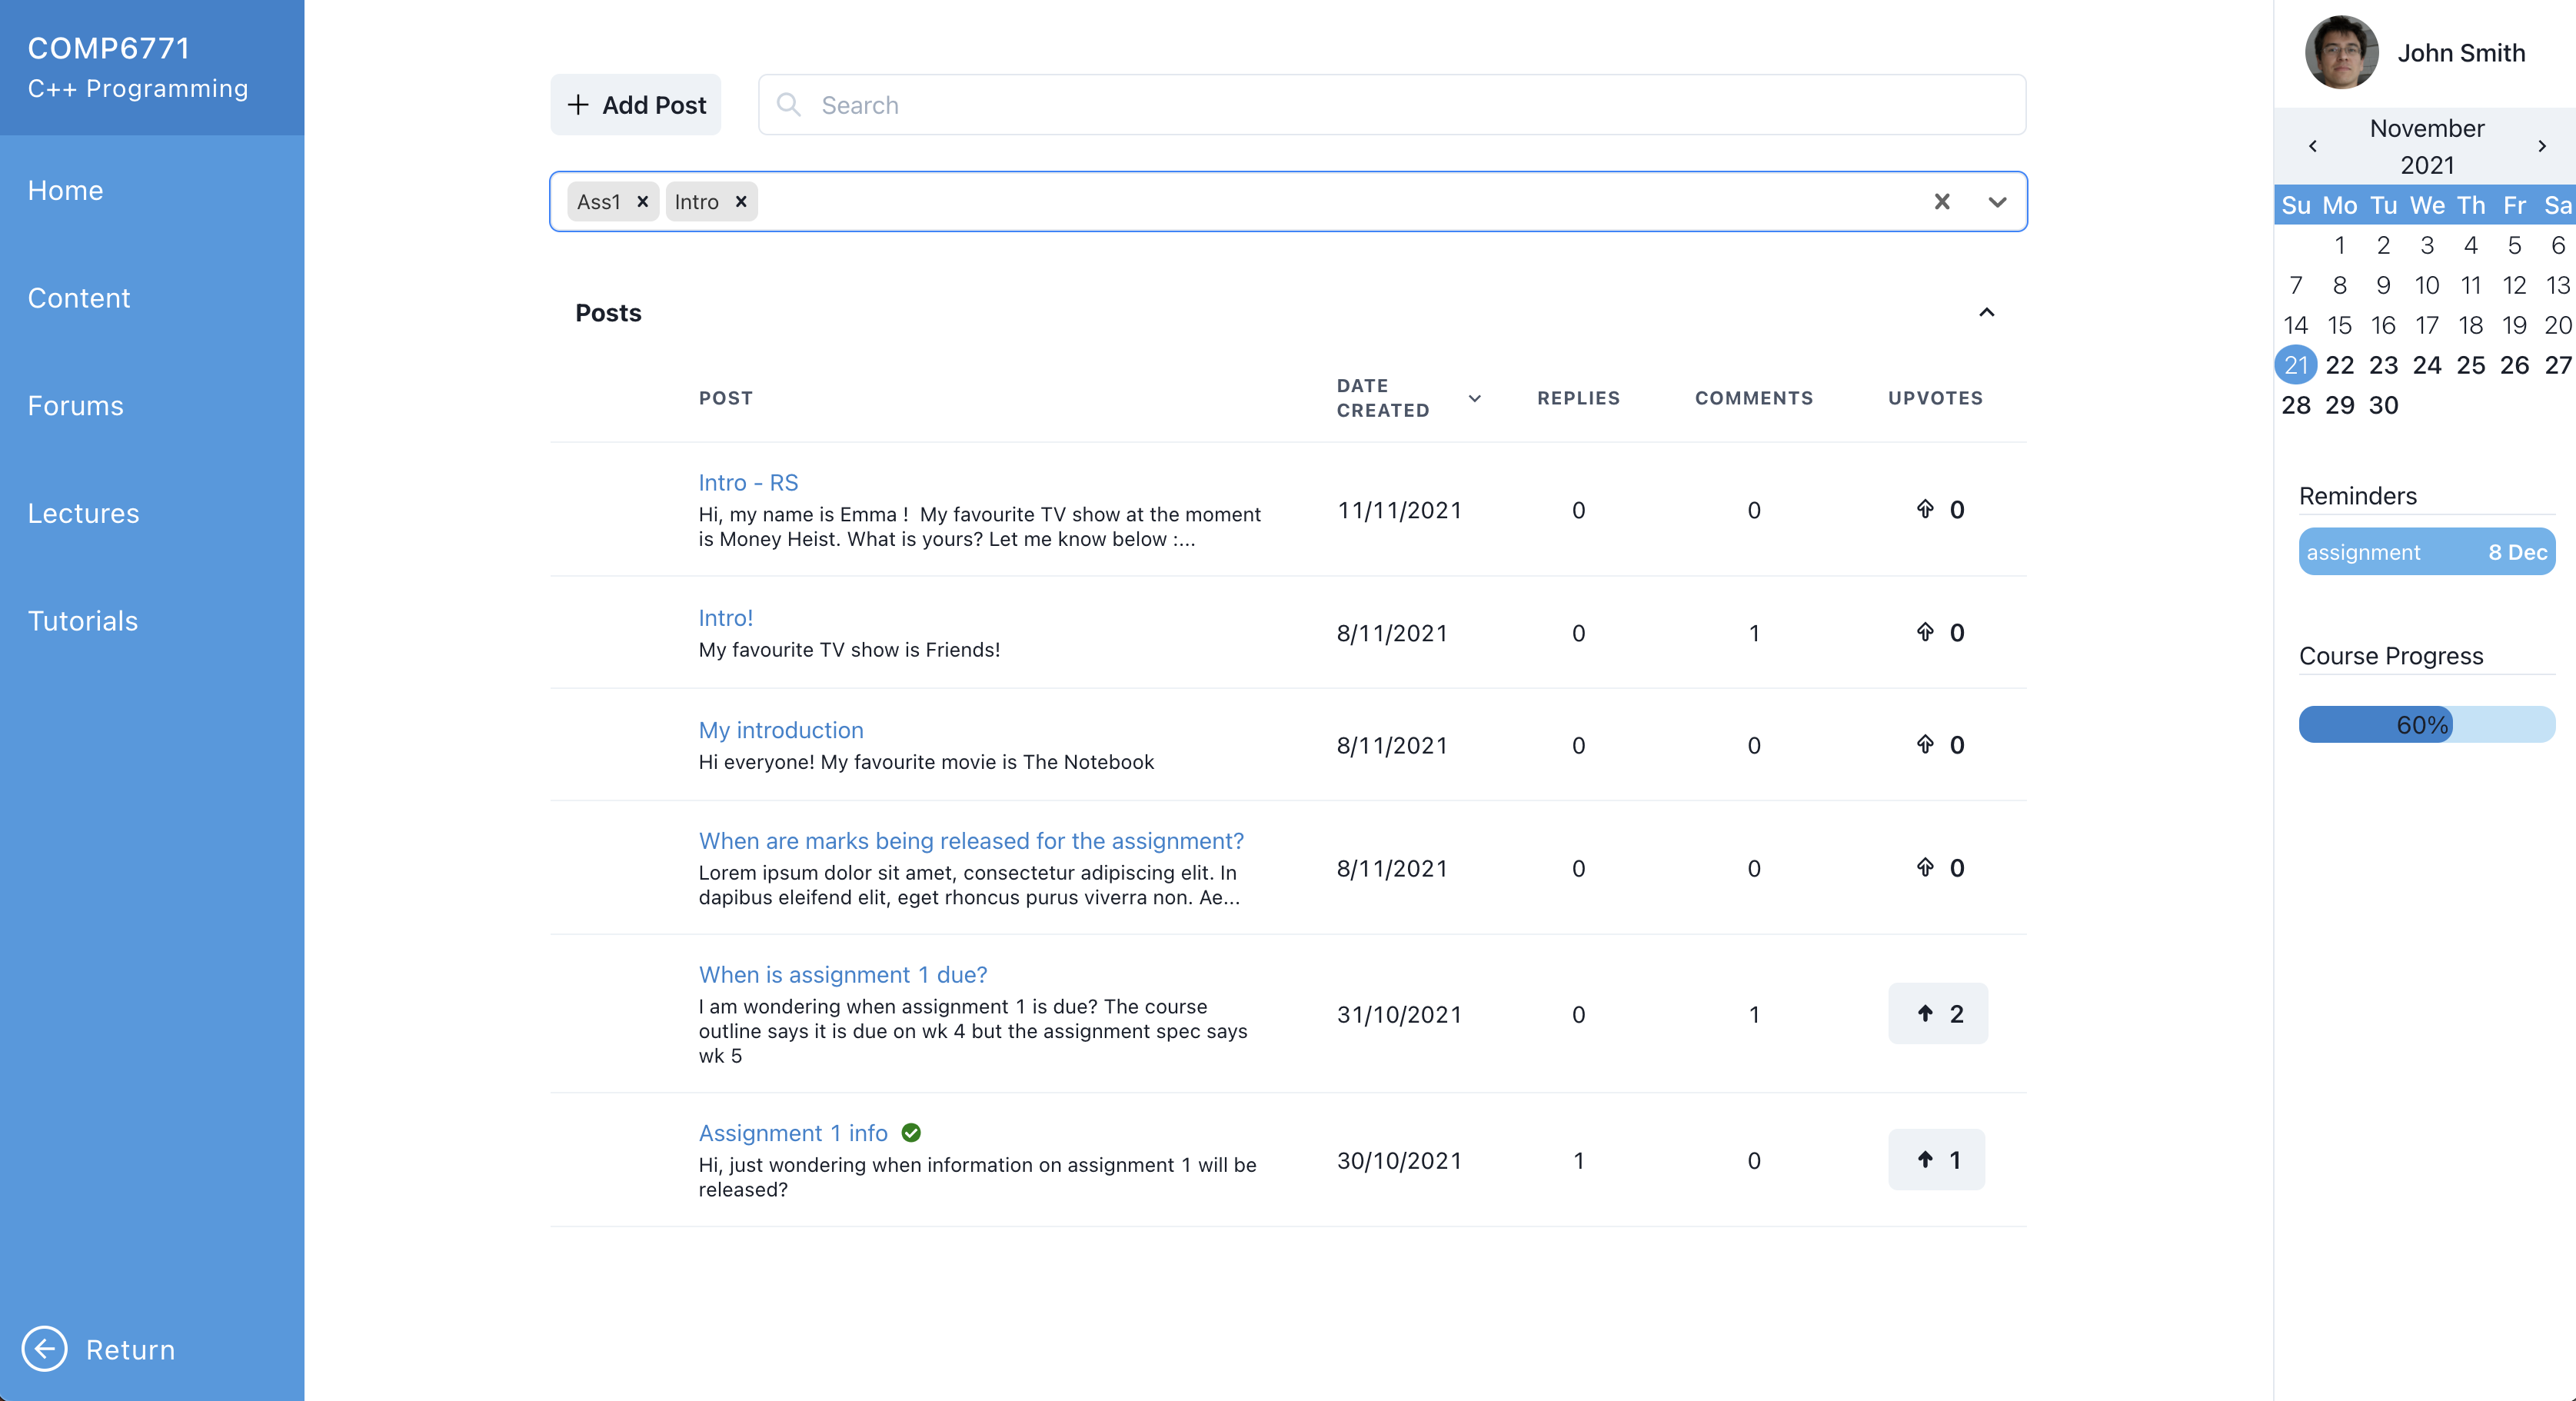
\includegraphics[scale=0.2]{forums-walkthrough-filter-results.png}
    \centering
    \caption{Filter results when filtering by tags ``Ass1" and ``Intro"}
\end{figure}

\subsubsection{How It Was Implemented}
When the user types a search term and hits ``enter", the search term is passed to the backend where a query to the database is made.
Since it directly queries the database, the search functionality is very basic.
If a user inputs more than one word, only posts that have a title or description that contains the exact search term will be returned.
There is also a small bug where the user has to clear the search bar and hit ``enter" again in order to re-render the original posts.

The filter uses the same \texttt{react-select} library mentioned previously.
If the user chooses to filter by tag, then the backend simply returns a list of all posts that have the corresponding tag.
When filtering by multiple tags at once, the posts returned from the backend are those that have any of the tags chosen.
For filtering by posts linked to announcements, the backend looks for posts with the ``Announcement" tag.
For the remainder of the pre-defined filters, the posts aren't explicitly tagged with them so there is logic built into the backend to handle these requests.
When filtering by ``answered" or ``unanswered" posts, the backend queries the number of comments and replies each post has.
For endorsed posts, the backend looks for posts with the \texttt{isEndorsed} flag.

\subsubsection{Considerations}
Instead of being hidden in a menu on the side or top of the forums, the search and filter options were placed at the top of the page to make it easy to find and interact with.
Due to time constraints, the search bar bug was unable to be fixed however, the search functionality itself isn't impacted too much by this.
A drop down menu was used for the filter to assist users who aren't quite sure what they're looking for however, the option to type directly into the bar is also available for users who know what they want.

\subsection{Post Page}
A user can click on a post title on the forum overview page to open the individual page for that post.

\begin{figure}[h!]
    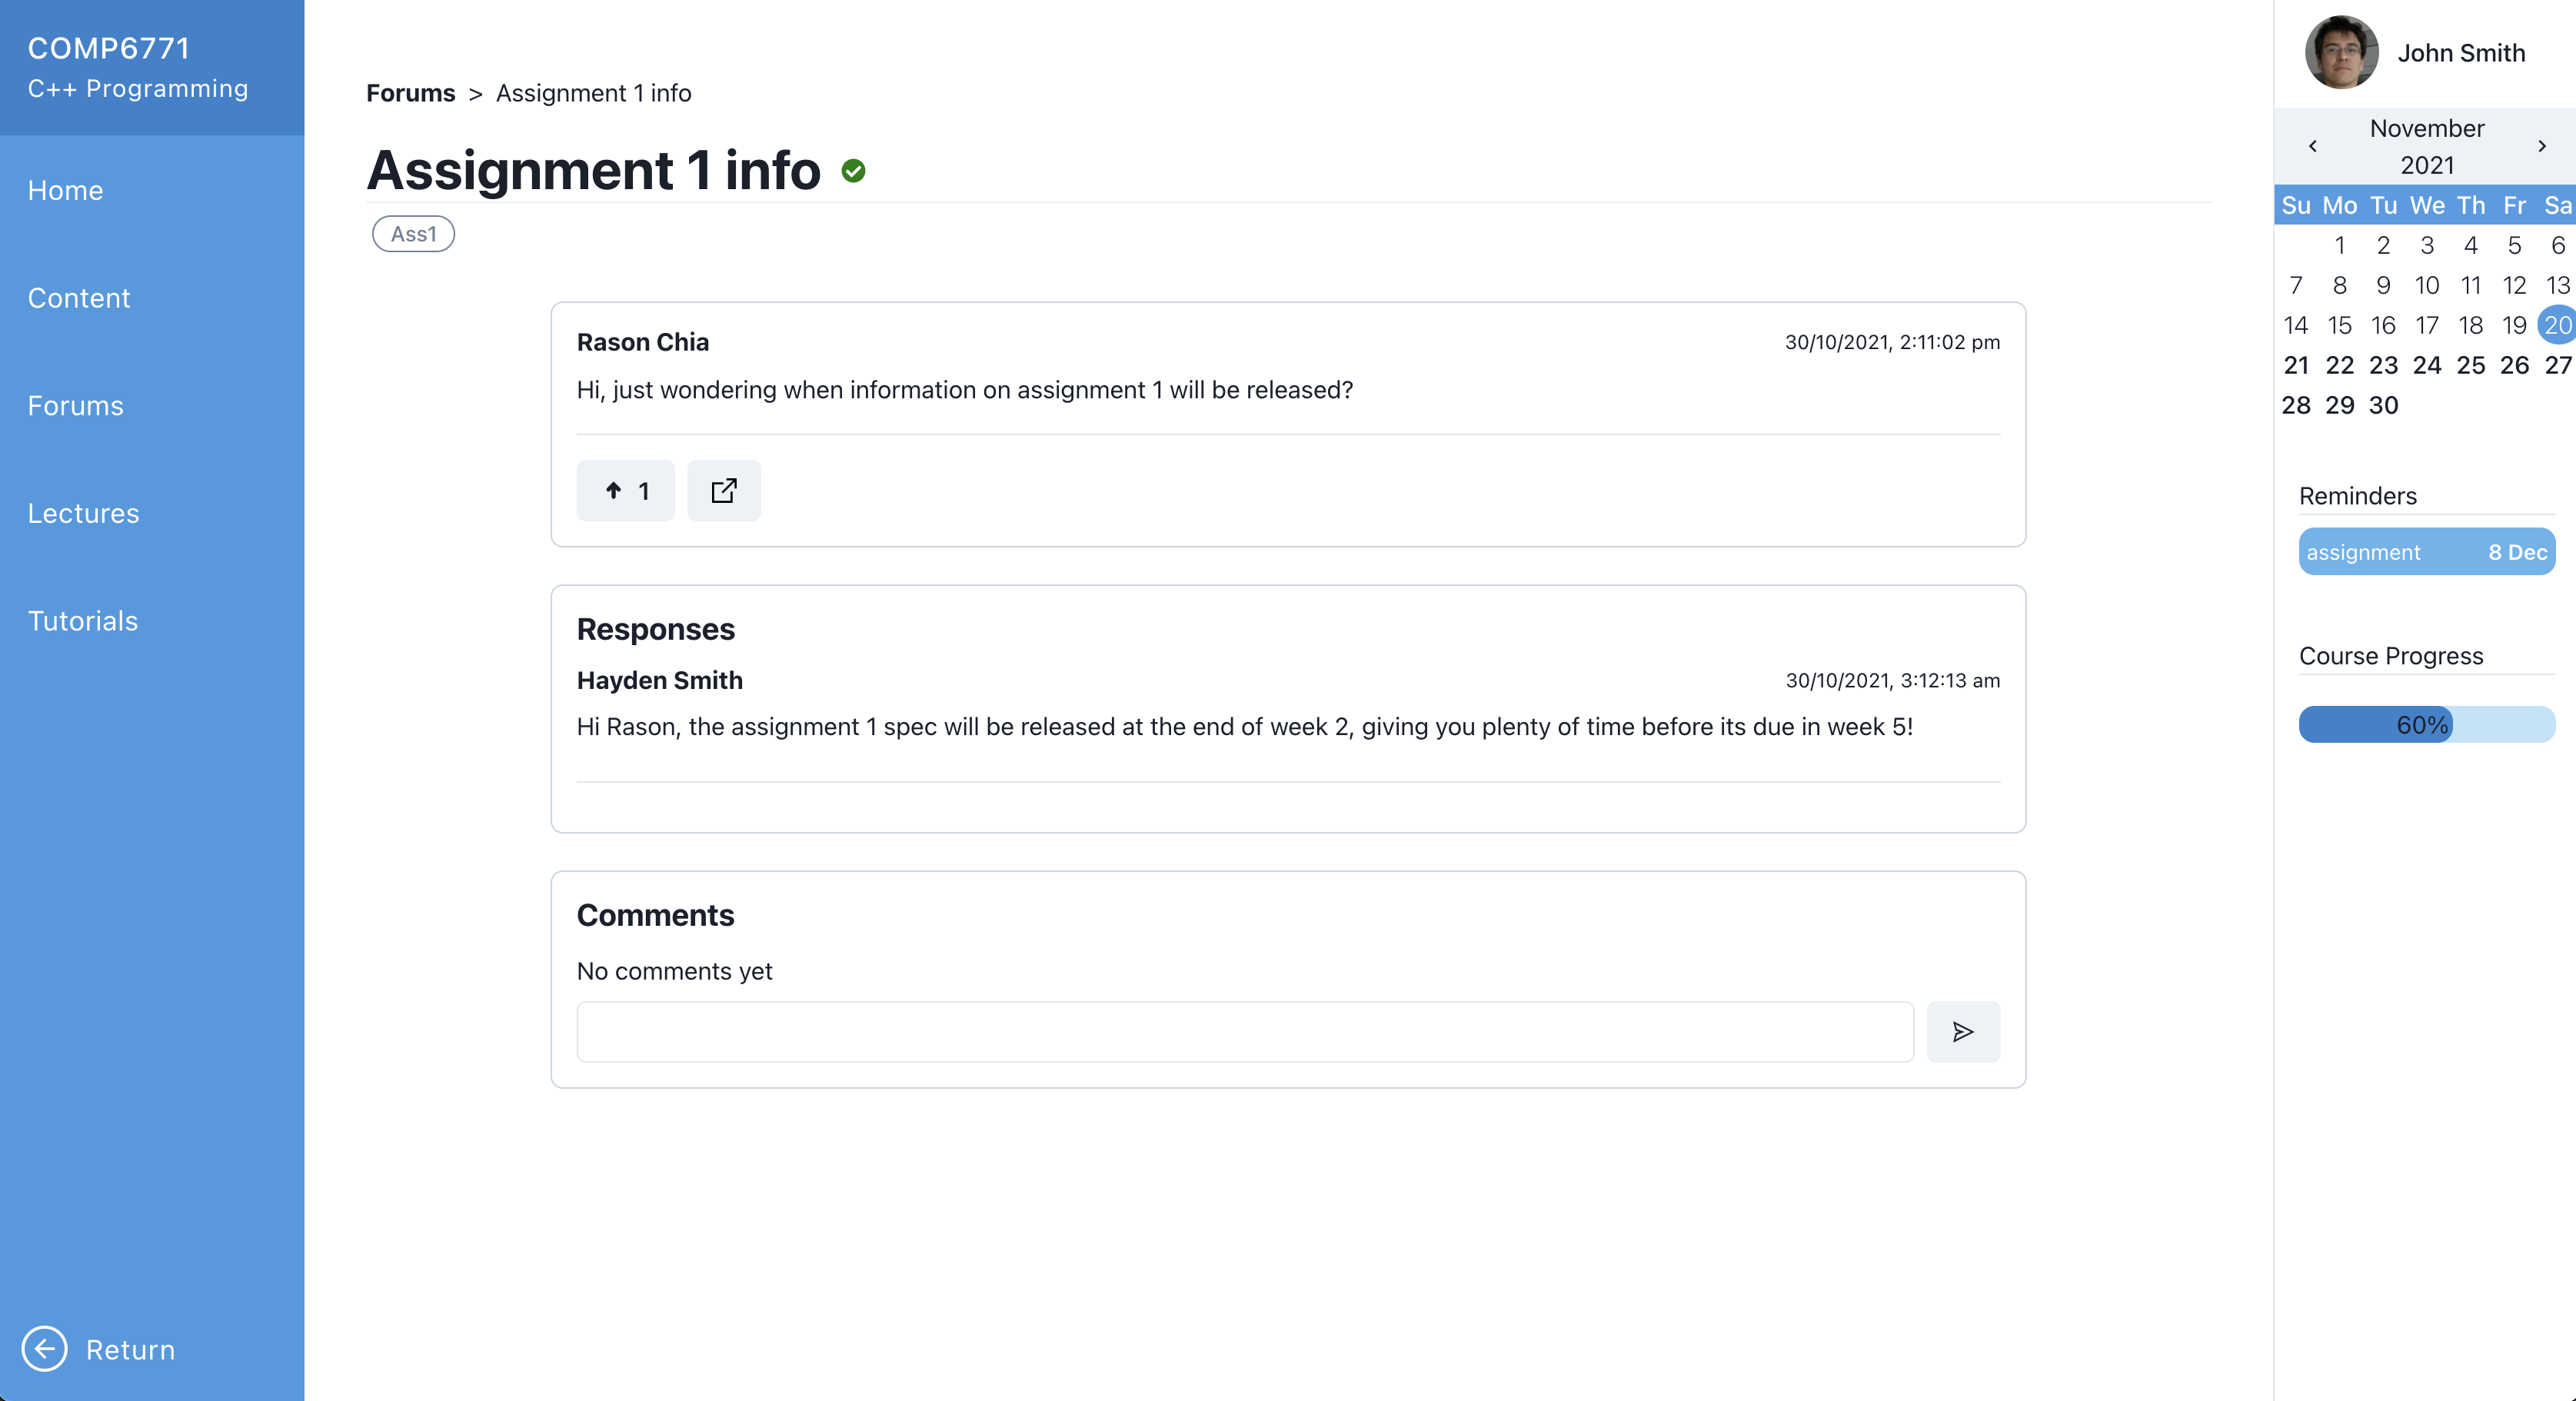
\includegraphics[scale=0.2]{forums-walkthrough-post-page.png}
    \centering
    \caption{Forum post page.}
\end{figure}

\subsubsection{Purpose}
Allows users to see all the post details, replies and comments in one place.
From this page, users can interact with the post by upvoting or sharing.
Upvoting allow users to like posts to draw attention to them.
The share button makes it easy for users to send a direct link to the post to others.
Depending on whether or not a user is staff, they can also leave a response and/or comment.

\subsubsection{What Was Implemented}
The top of the post page has links to navigate back to the forum overview page.
Underneath that is the post title and tags.
If the post has been endorsed by staff, there will be a green check mark next to the post title.
If users are unsure of what the green check mark means, they can hover over it for an explanation.

\begin{figure}[h!]
    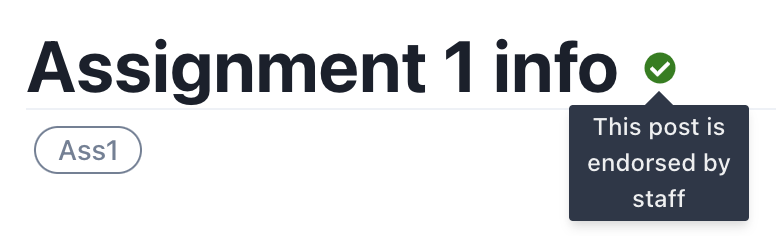
\includegraphics[scale=0.5]{forums-walkthrough-endrosed-tooltip.png}
    \centering
    \caption{Tooltip explaining endorsed icon.}
\end{figure}

The post page is then split into three sections.
The first is the post details which contains the author, date and time created, and post description.
There are also buttons to upvote and share the post.
The second and third sections contain all the responses and comments for the post.
Similar to the post details section, each response and comment also displays the author and timestamp.

\subsubsection{How It Was Implemented}
When navigating to the post page, the \texttt{id} of the post is used to display the correct data from the backend.
This same call is also used to populate the responses and comments for the post.

When a user clicks the upvote button to like a post, a backend call is made to increment the value and add the user to the list of upvoters.
This ensures that users can't upvote the same post more than once.
It also allows the frontend to rerender the button with the updated number of upvoters, and change the icon to the filled in arrow.
Similarly, the user can click the upvote button to remove their upvote which makes a backend call to decrement the value and remove them from the upvoters list.

\begin{figure}[h!]
    
\includegraphics[scale=0.5]{forums-walkthrough-upvote-buttons.png}
    \centering
    \caption{Upvote buttons that have and haven't been liked.}
\end{figure}

If a user clicks the share button, the url of the page is directly copied to their clipboard.
A toast element shows to confirm that the link has been clicked

\begin{figure}[h!]
    
\includegraphics[scale=0.5]{forums-walkthrough-copied-link.png}
    \centering
    \caption{Toast to confirm that post link has be copied.}
\end{figure}

\subsubsection{Considerations}
Initially, an endorsed post was marked by the messaging \textit{``This post is endorsed by staff"} which showed under the post content.

\begin{figure}[h!]
    
\includegraphics[scale=0.5]{forums-walkthrough-old-endorsed-messaging.png}
    \centering
    \caption{Old endorsed messaging on forum posts.}
\end{figure}

There was a concern with this taking up too much vertical space so now, the messaging has been removed and only the endorsed icon shows next to the post title.
The tooltip for the endorsed icon was added however, to ensure that a user could easily find out what the symbol meant if they were unsure.

By splitting the page into three sections with obvious borders, users can easily scan the post page and find what they're looking for.
It was an early design decision to create separate responses and comments section.
The idea was to only allow staff members to post in the responses section.
This is to make it easy for students to find exactly where the most reliable answer to a question may be.
It also ensures that staff members can find what posts haven't been replied to and require their attention.
The comments section gives students a place to answer a post themselves or leave a follow up question.

It was decided that the upvote button would only show the number of upvotes, and not the names of the upvoters, so that students can remain anonymous when liking a post.
Hopefully, students will feel more comfortable using this feature since no one will know exactly who upvoted a post.

\newpage

\subsection{Edit and Delete Post}
If the logged in user is the author of the post, they will see additional buttons on the post page to edit or delete their post.

\begin{figure}[h!]
    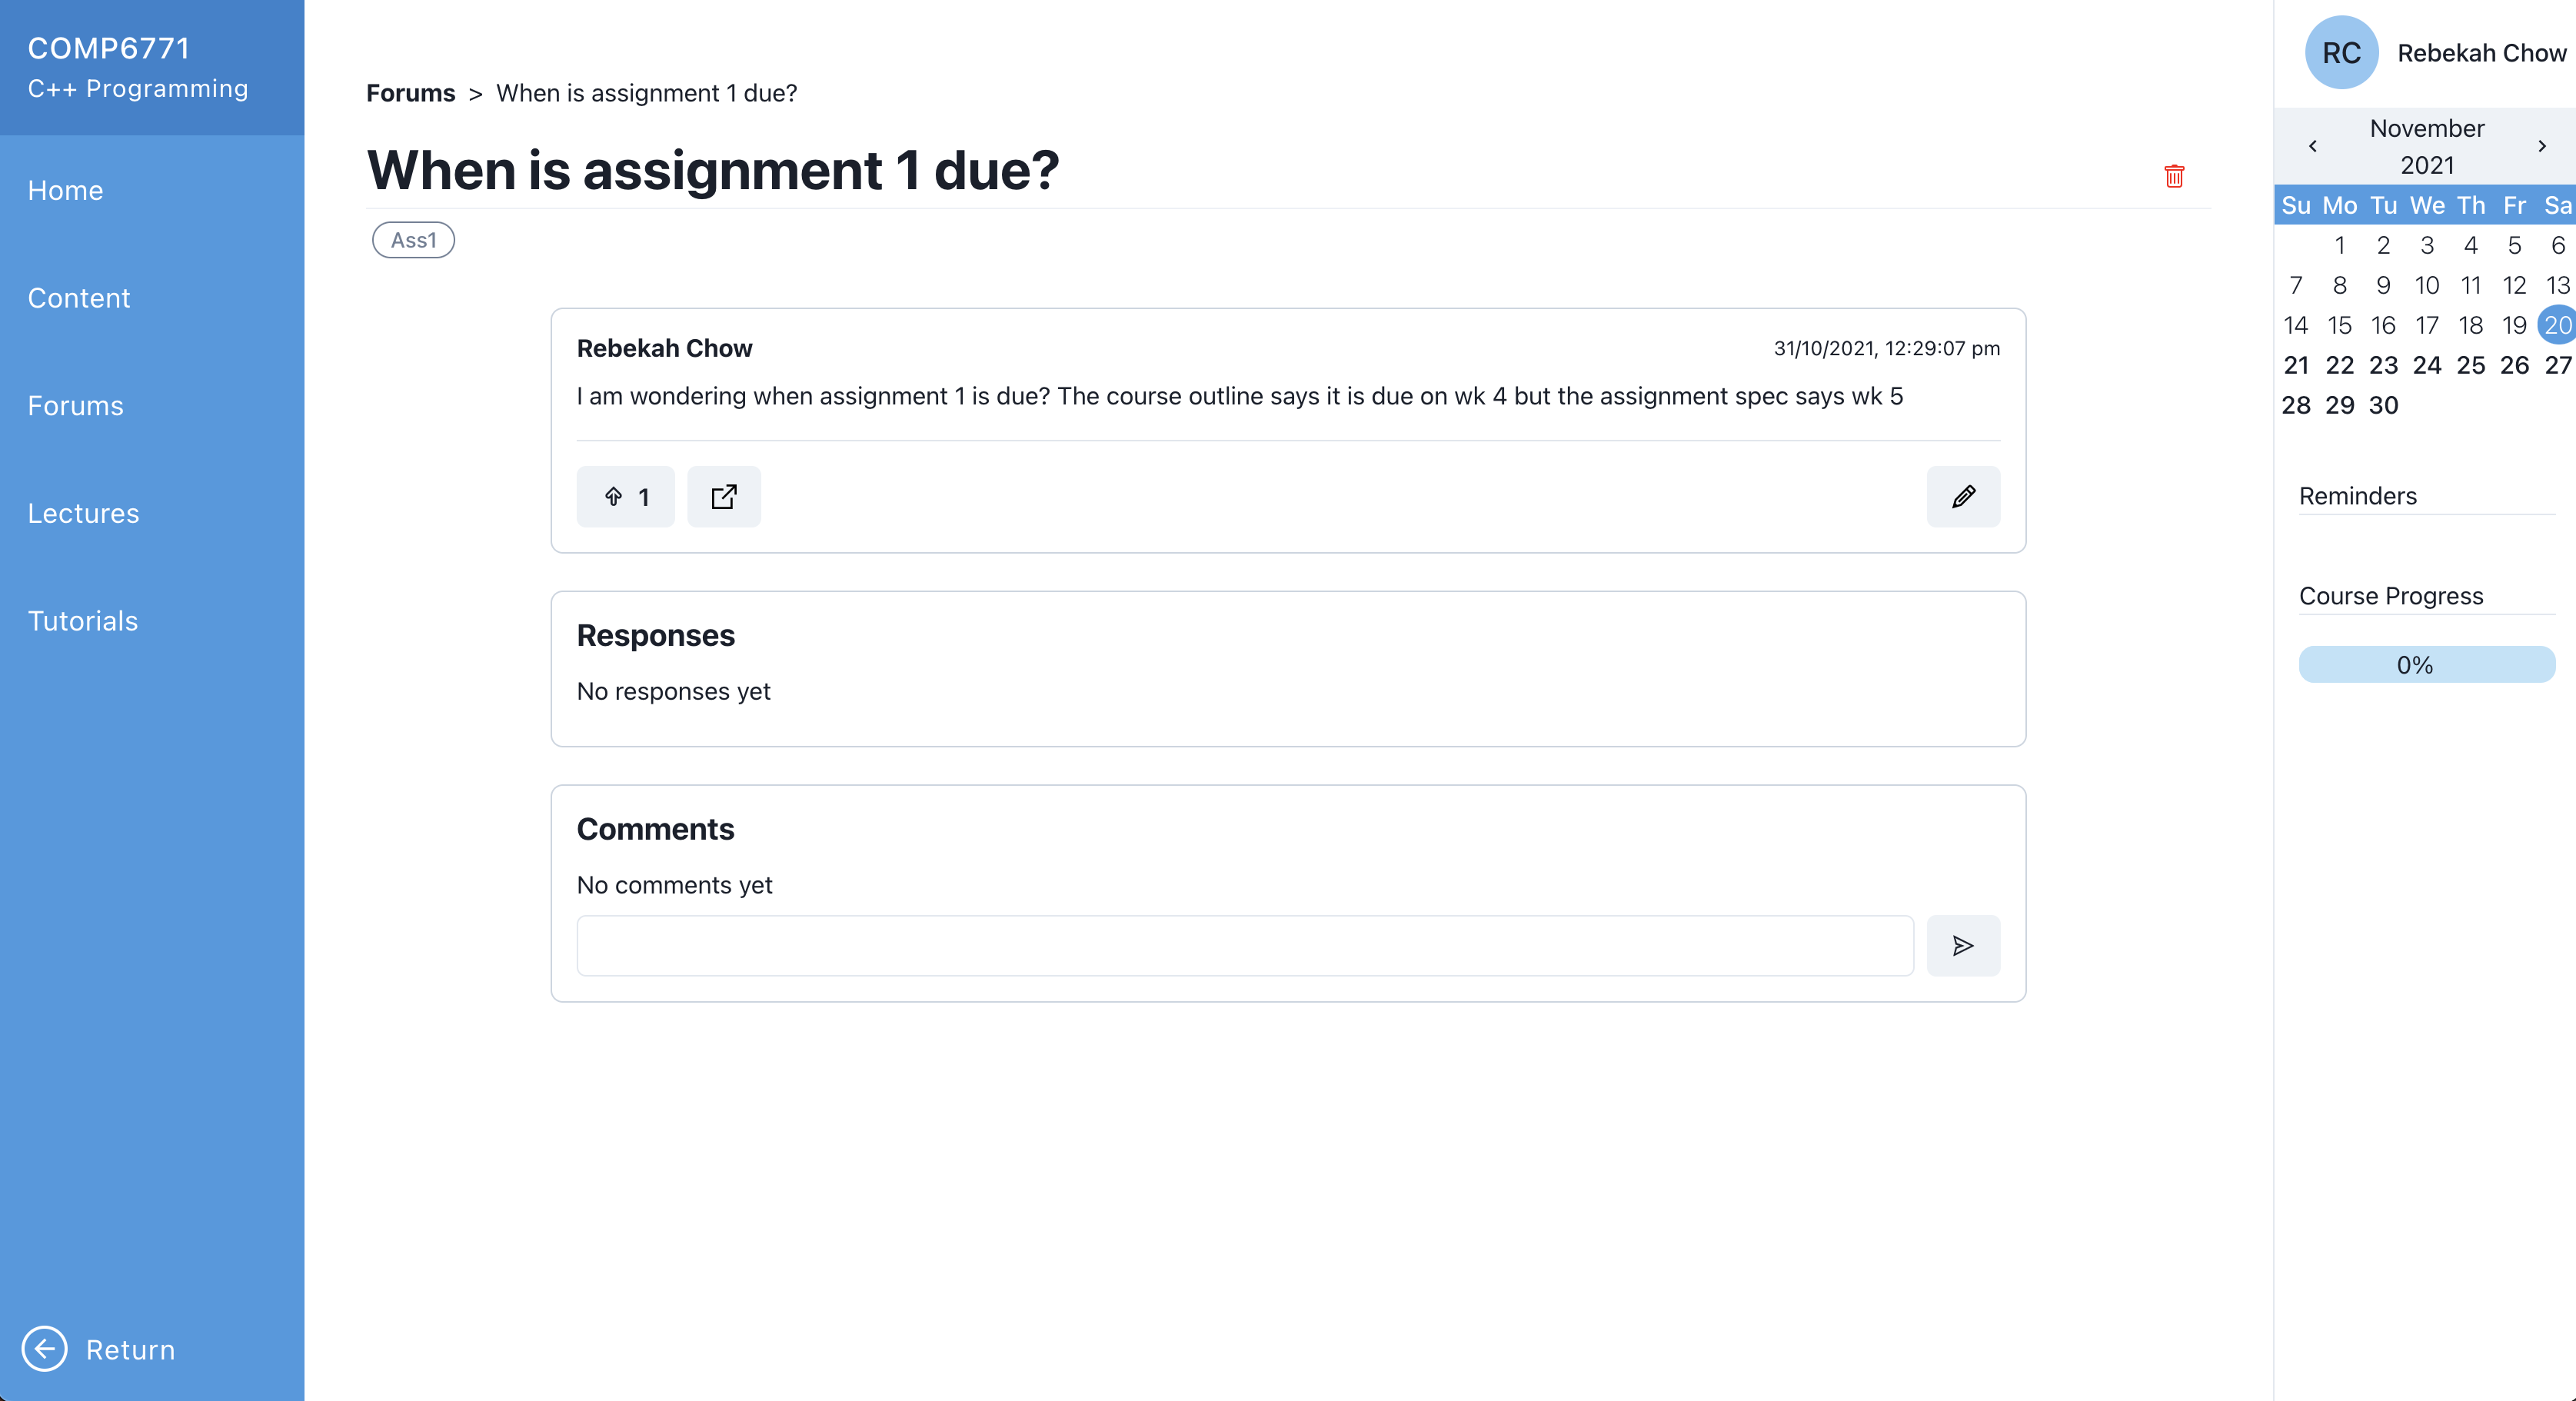
\includegraphics[scale=0.2]{forums-walkthrough-edit-delete.png}
    \centering
    \caption{Forum post page when the logged in user is the author of the post.}
\end{figure}

\subsubsection{Purpose}
To allow users to easily make changes to their post or delete their post.

\subsubsection{What Was Implemented}
When viewing one of their own posts, a user would be able to see the delete icon in the top right corner.
Clicking this button will show a confirmation message to ensure that the user definitely wants to delete their post.
Once confirmed, the post will be deleted and the user will be navigated back to the forum overview page.

\begin{figure}[h!]
    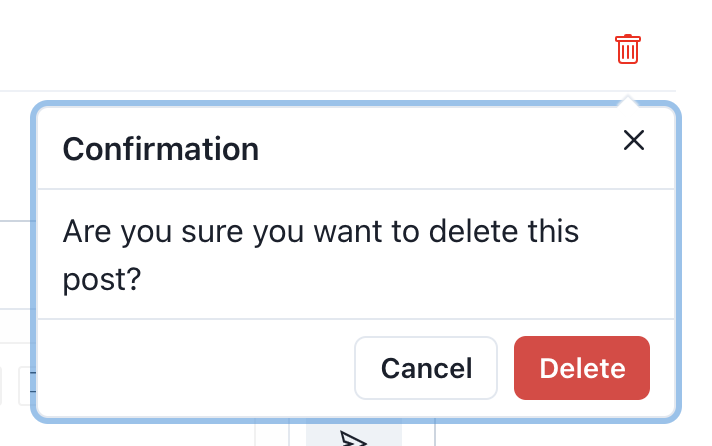
\includegraphics[scale=0.5]{forums-walkthrough-delete-confirmation.png}
    \centering
    \caption{Confirmation messaging for deleting a post.}
\end{figure}

To edit a post, there is an edit button on the bottom right of the post details section of the page.
Clicking this button will show the rich text editor and allow users to edit their post description.
Saving the changes will automatically update the page.

\begin{figure}[h!]
    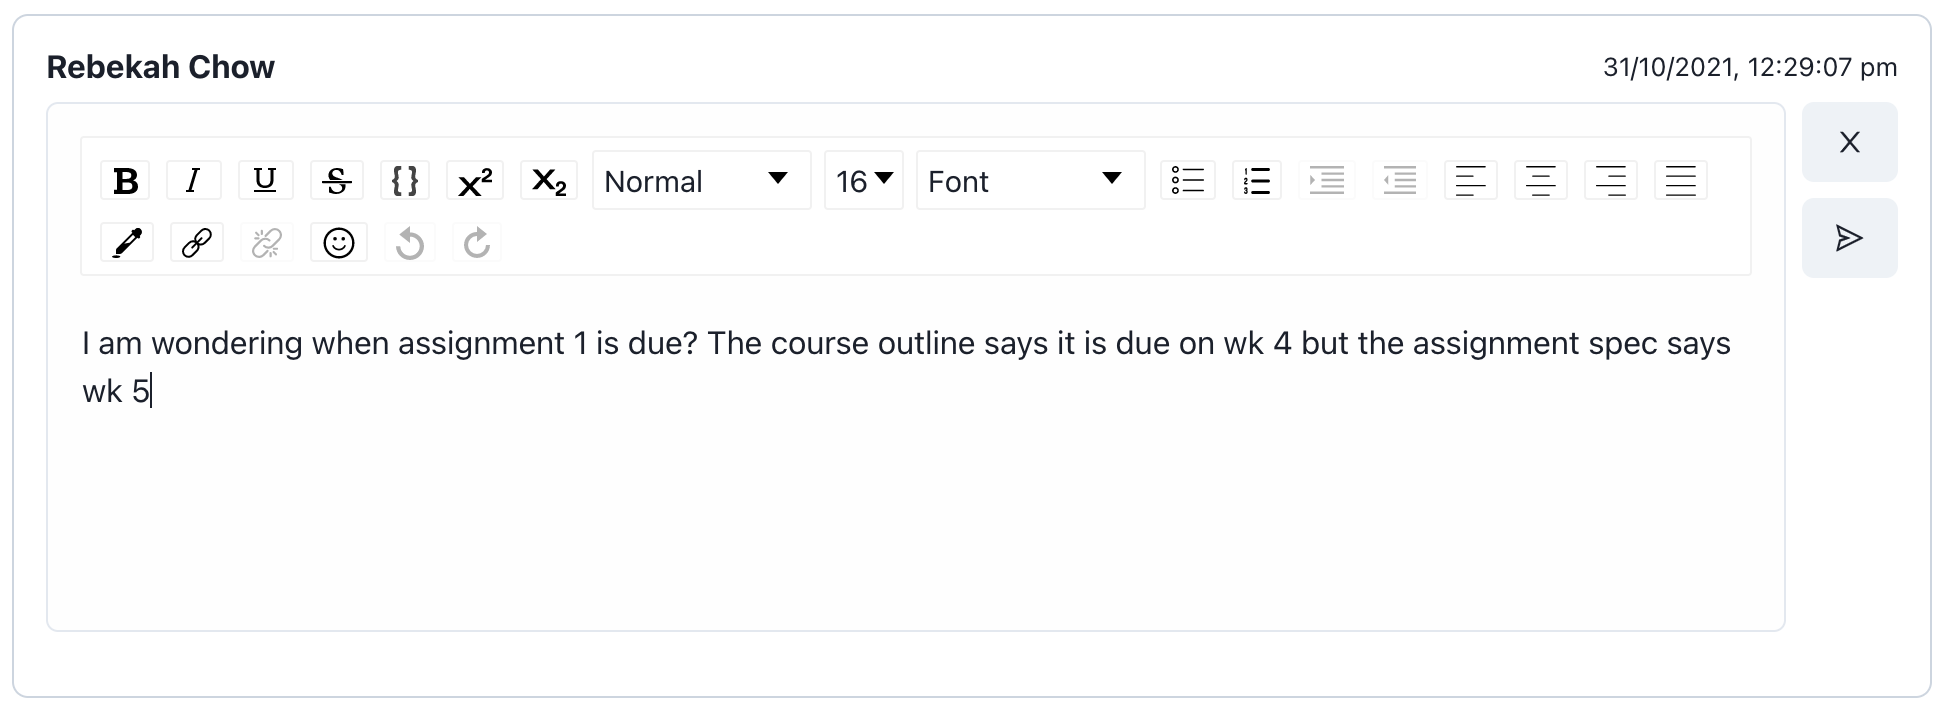
\includegraphics[scale=0.3]{forums-walkthrough-edit-post.png}
    \centering
    \caption{Interface to edit post.}
\end{figure}

\subsubsection{How It Was Implemented}
When deleting a post, a backend call is made to remove it from the database.

When editing a post, the draft editor component will be initialised with the existing post content.
As the user types, the state of the editor will be updated so that when the user saves their change, the backend will be updated immediately.
This ensures that the frontend is also updated instantly.

\subsubsection{Considerations}
The confirmation message for deleting was added to ensure that posts weren't accidentally deleted because of incorrect clicks.

It was decided that the editor would open in the post details section when editing a post so that users aren't navigated elsewhere to make changes, providing the simplest user experience.

\subsection{Comment}
A user can click the input box in the comments section to open the rich text editor and leave a comment.

\newpage

\begin{figure}[h!]
    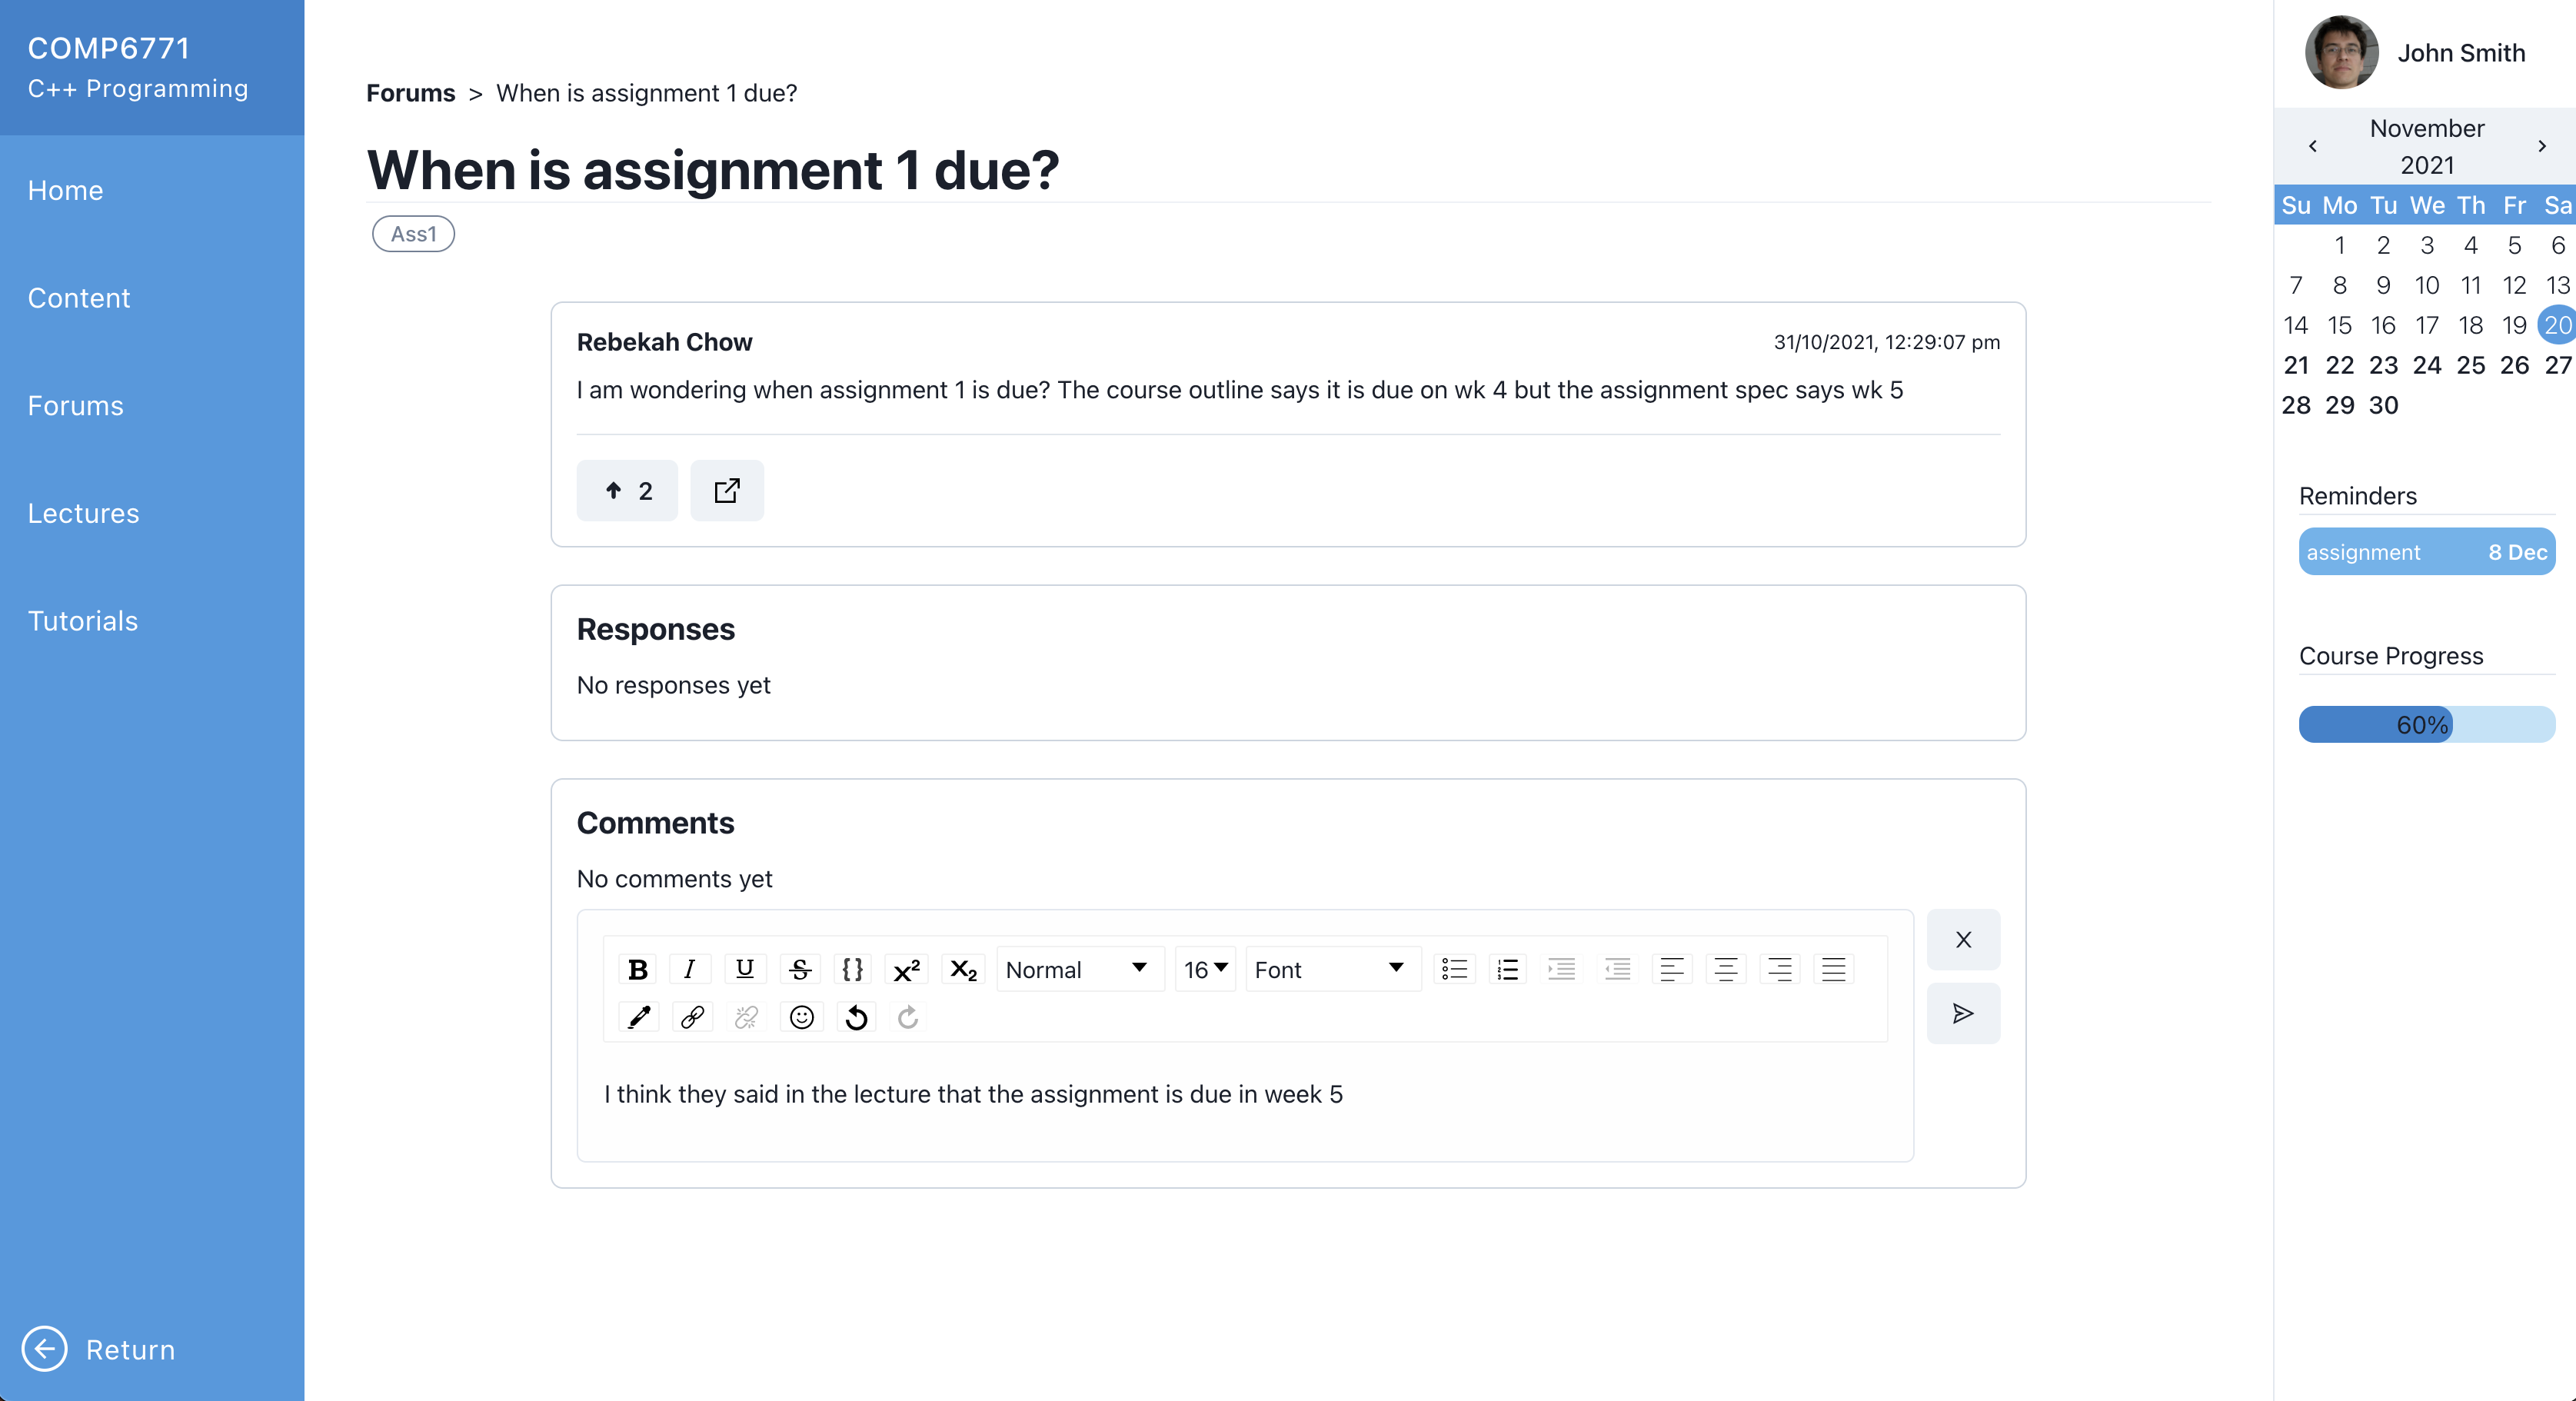
\includegraphics[scale=0.2]{forums-walkthrough-comment.png}
    \centering
    \caption{Leaving a comment on a forum post.}
\end{figure}

\subsubsection{Purpose}
Gives students a dedicated area to answer forum posts themselves or leave follow-up questions.

\subsubsection{What Was Implemented}
By default, the page shows a simple input field in the comments section.
When a user clicks on it, it opens the rich-text editor so that they have formatting options for their comment.
A user can either close the rich-text editor to cancel leaving a comment, in which case the rich-text editor will close and be replaced with the simple input field.
Otherwise, the comments section will automatically be updated with the user's comment when they hit ``Save".

\begin{figure}[h!]
    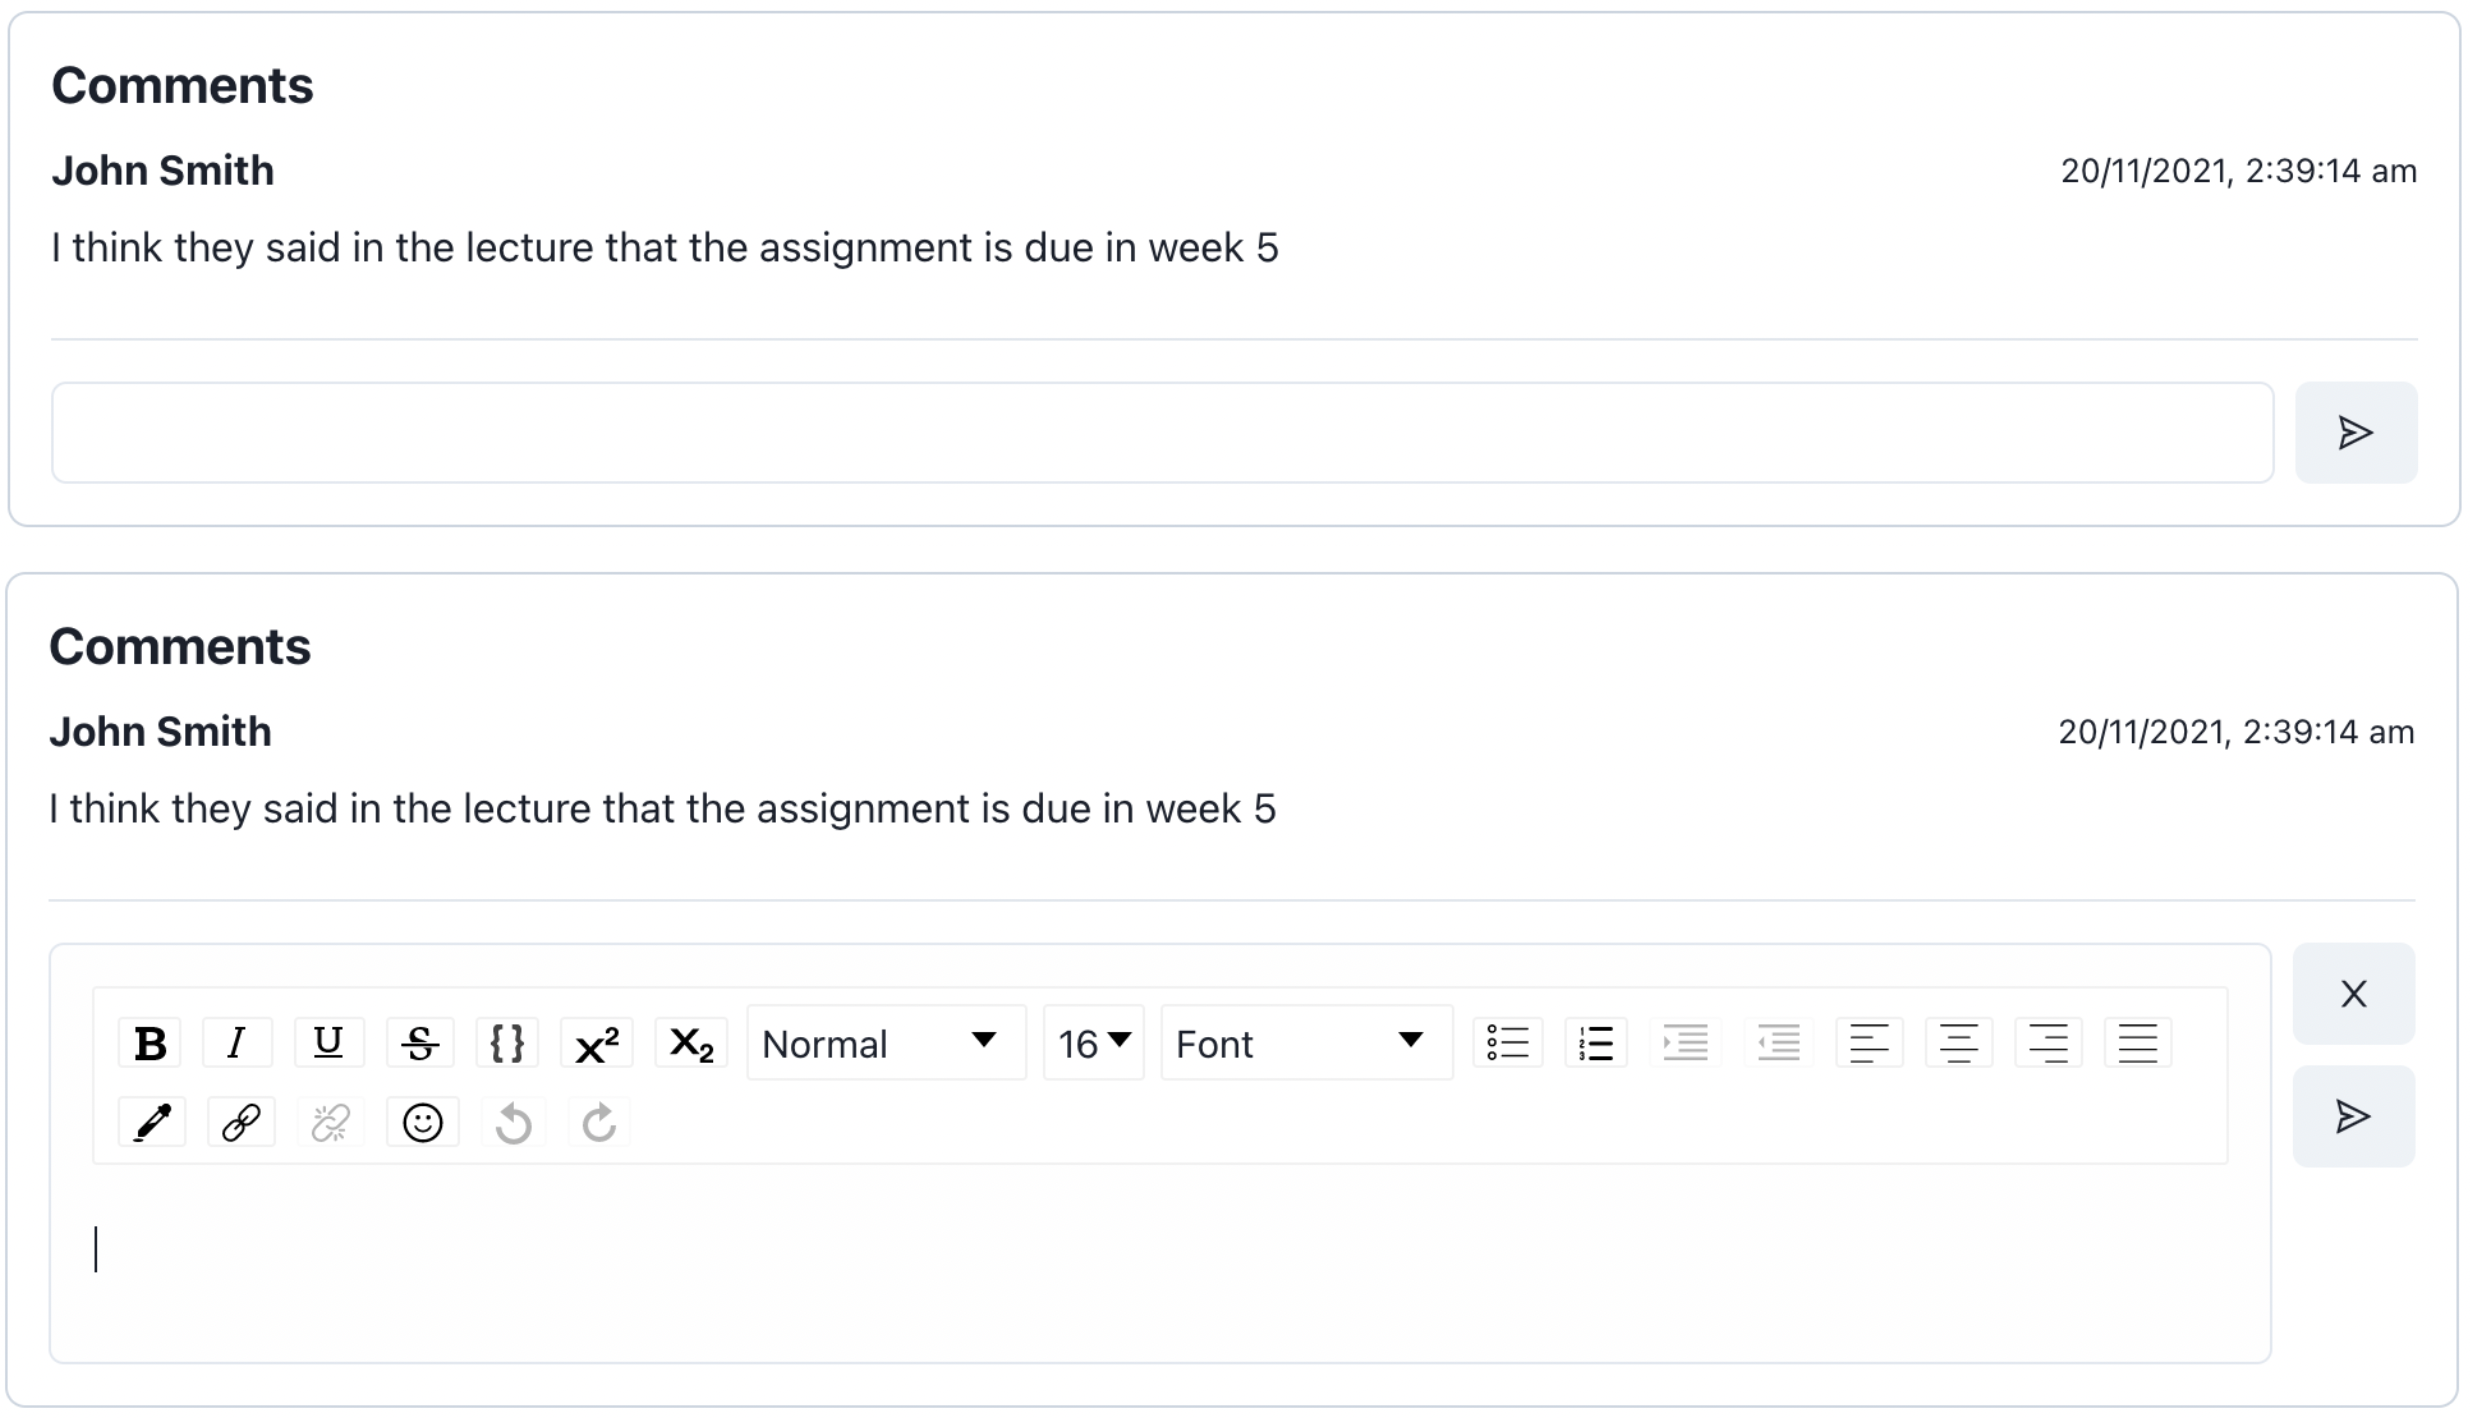
\includegraphics[scale=0.2]{forums-walkthrough-comments-inputs.png}
    \centering
    \caption{Clicking on the input field will open the rich-text editor.}
\end{figure}

If the logged in user is the author of a comment, they will see additional buttons that allow them to edit or delete a comment.

\begin{figure}[h!]
    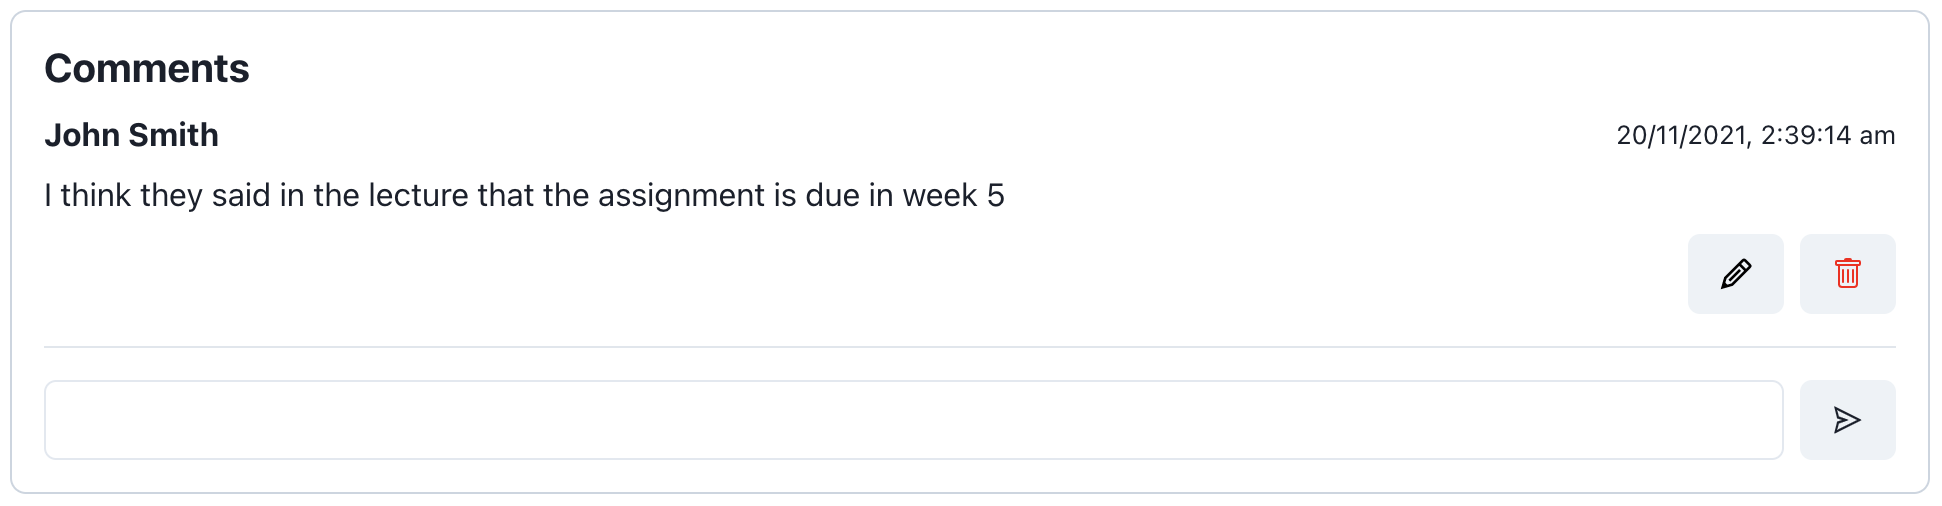
\includegraphics[scale=0.3]{forums-walkthrough-comments-edit-delete.png}
    \centering
    \caption{Comment with edit and delete options.}
\end{figure}

This works very similarly to editing and deleting a post.
Editing a comment will open a rich-text editor with the existing comment so user's can make changes.
Deleting a comment will ask for the user's confirmation before deleting the comment from the database.

\subsubsection{How It Was Implemented}
Similar to editing a post, the draft editor component is initialised when the simple input field is clicked.
The user's input is stored as they type and sent to the backend once they hit ``Send".
This causes the frontend to re-render so that the comment instantly shows on the post page.

Additionally, the implementation for editing and deleting a comment is the exact same as editing and deleting a post.

\subsubsection{Considerations}
The flow for editing and deleting a comment was kept as similar to editing and deleting a post as possible to reduce the amount of learning a user has to do when first interacting with the system.
By keeping the implementation relatively the same, and using icons that are typically associated with editing and deleting, users can easily work out how to complete these actions.

\subsection{Manage Tags}
Users who have a staff account will see a ``Manage Tags" button on the top right corner that, when clicked, opens up the ``Manage Tags" modal.

\begin{figure}[h!]
    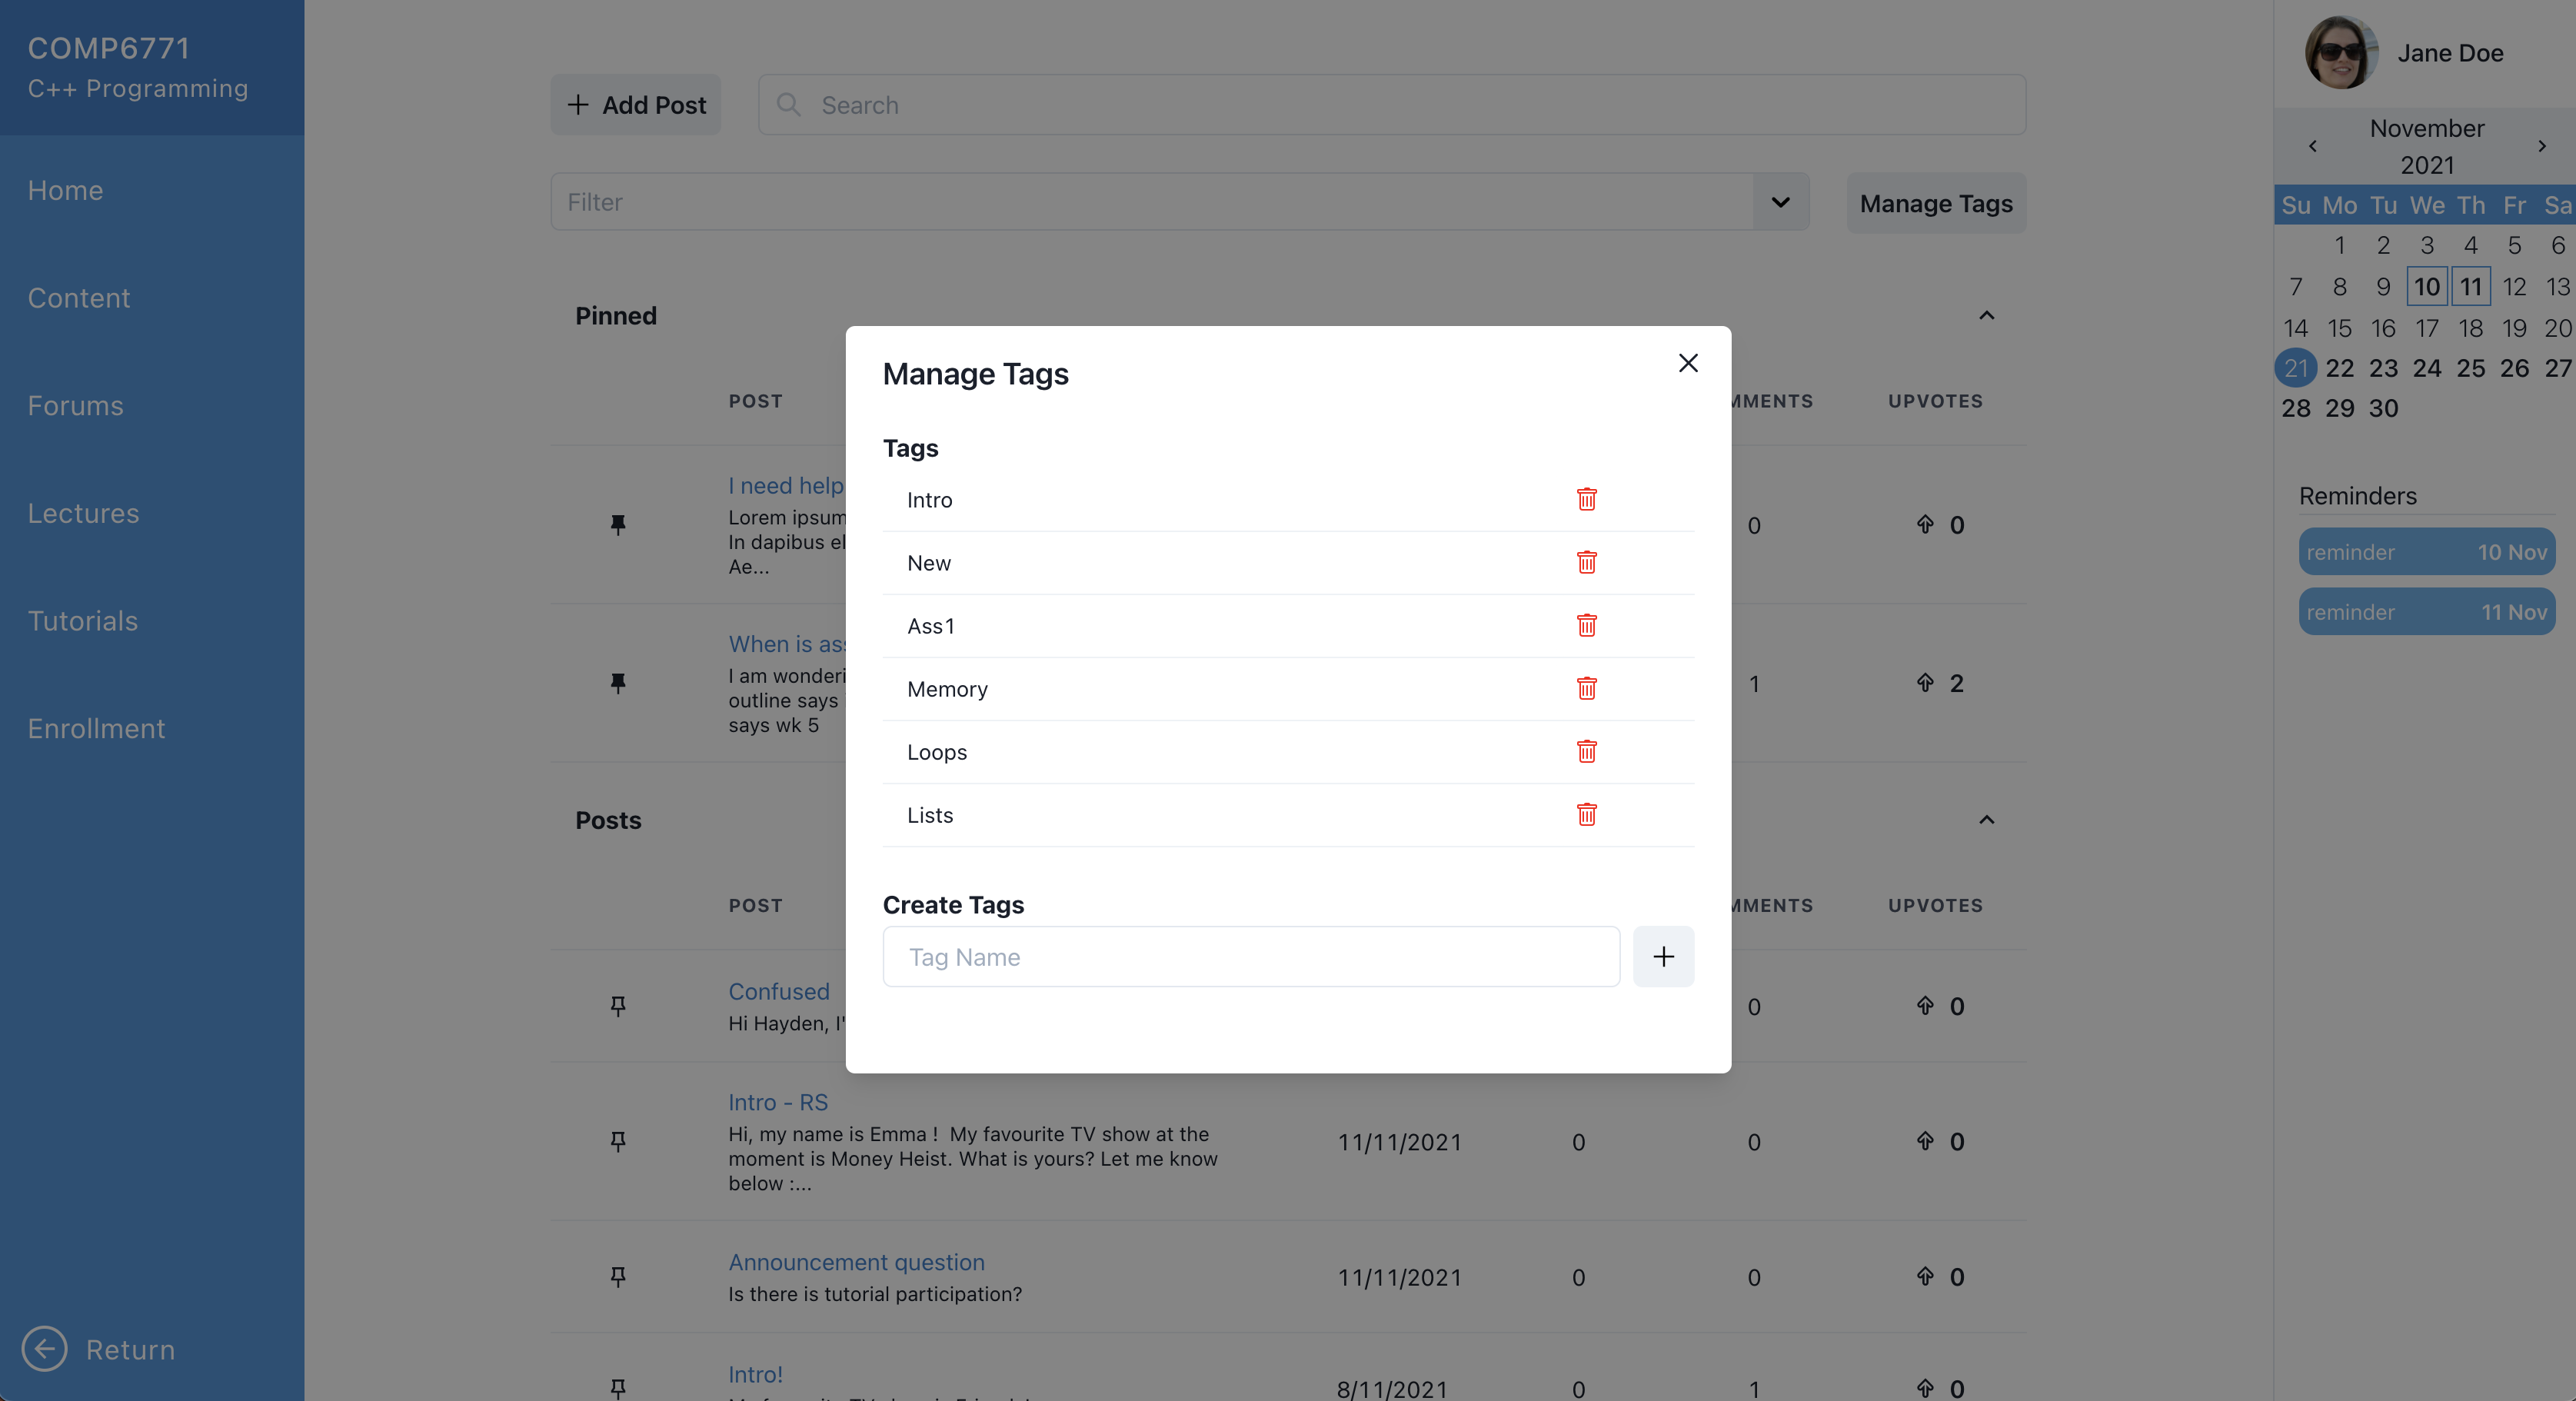
\includegraphics[scale=0.2]{forums-walkthrough-manage-tags.png}
    \centering
    \caption{Manage tags modal.}
\end{figure}

\subsubsection{Purpose}
Allows staff users to see all the tags for a course, create new tags and delete tags.
Tags are useful for categorising and filtering through posts.

\subsubsection{What Was Implemented}
The ``Manage Tags" button sits at the top of the forum overview page, next to the filter.
When clicked, it opens the ``Manage Tags" modal which contains a list of all the tags that have been created for the topic group.
Next to each tag is a delete button that allows staff to delete the tag.
At the bottom of the modal, staff can type the name of a new tag and click the ``+" to add it to the list.

\subsubsection{How It Was Implemented}
When the modal is opened, a backend call is made to get a list of all the tags.
These are then displayed in a simple \texttt{table} component alongside a delete button for each tag.

Deleting a tag follows a similar flow to deleting a post or comment.
When the button is clicked, a confirmation message is displayed to ensure the user doesn't accidentally delete a tag.
Once confirmed, the tag is deleted from the database and removed from this list.

\newpage

\begin{figure}[h!]
    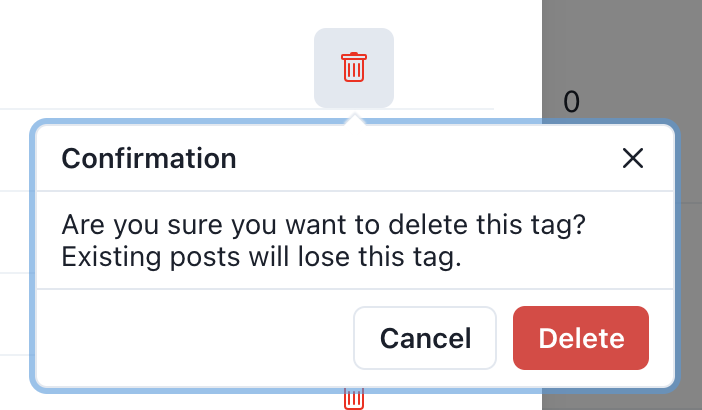
\includegraphics[scale=0.5]{forums-walkthrough-manage-tag-delete.png}
    \centering
    \caption{Deleting a tag.}
\end{figure}

A staff user can create a new tag by typing its name into the input field and clicking ``+".
This makes a backend call that adds the tag to the database and links it to the current topic group.
If a staff user tries to create a duplicate tag, the backend will return an error and the user will be informed.

\begin{figure}[h!]
    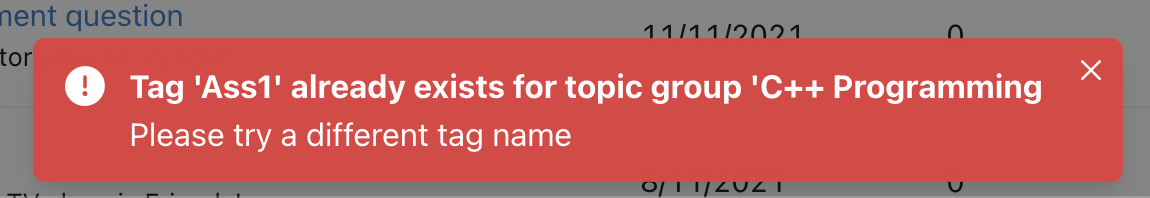
\includegraphics[scale=0.5]{forums-walkthrough-manage-tag-duplicate.png}
    \centering
    \caption{Error messaging when trying to create a duplicate tag.}
\end{figure}

Otherwise, a toast will show to confirm the tag has been created.

\begin{figure}[h!]
    
\includegraphics[scale=0.5]{forums-walkthrough-manage-tag-confirmation.png}
    \centering
    \caption{Confirmation messaging when creating a new tag.}
\end{figure}

\subsubsection{Considerations}
Similar to adding a post, a modal was used for managing tags to avoid users being navigated to a new page.
This keeps the flow as simple as possible.

In order to prevent the tags from becoming a bloated system and ensure that the functionality is useful for users, it was decided that only staff are allowed to create new tags.
This way, course staff don't have to worry about students creating unnecessary, inappropriate or redundant tags.

\subsection{Pinned Posts}
Staff users are able to pin posts to the top of the forum overview page by clicking the pin icon in the posts table.

\begin{figure}[h!]
    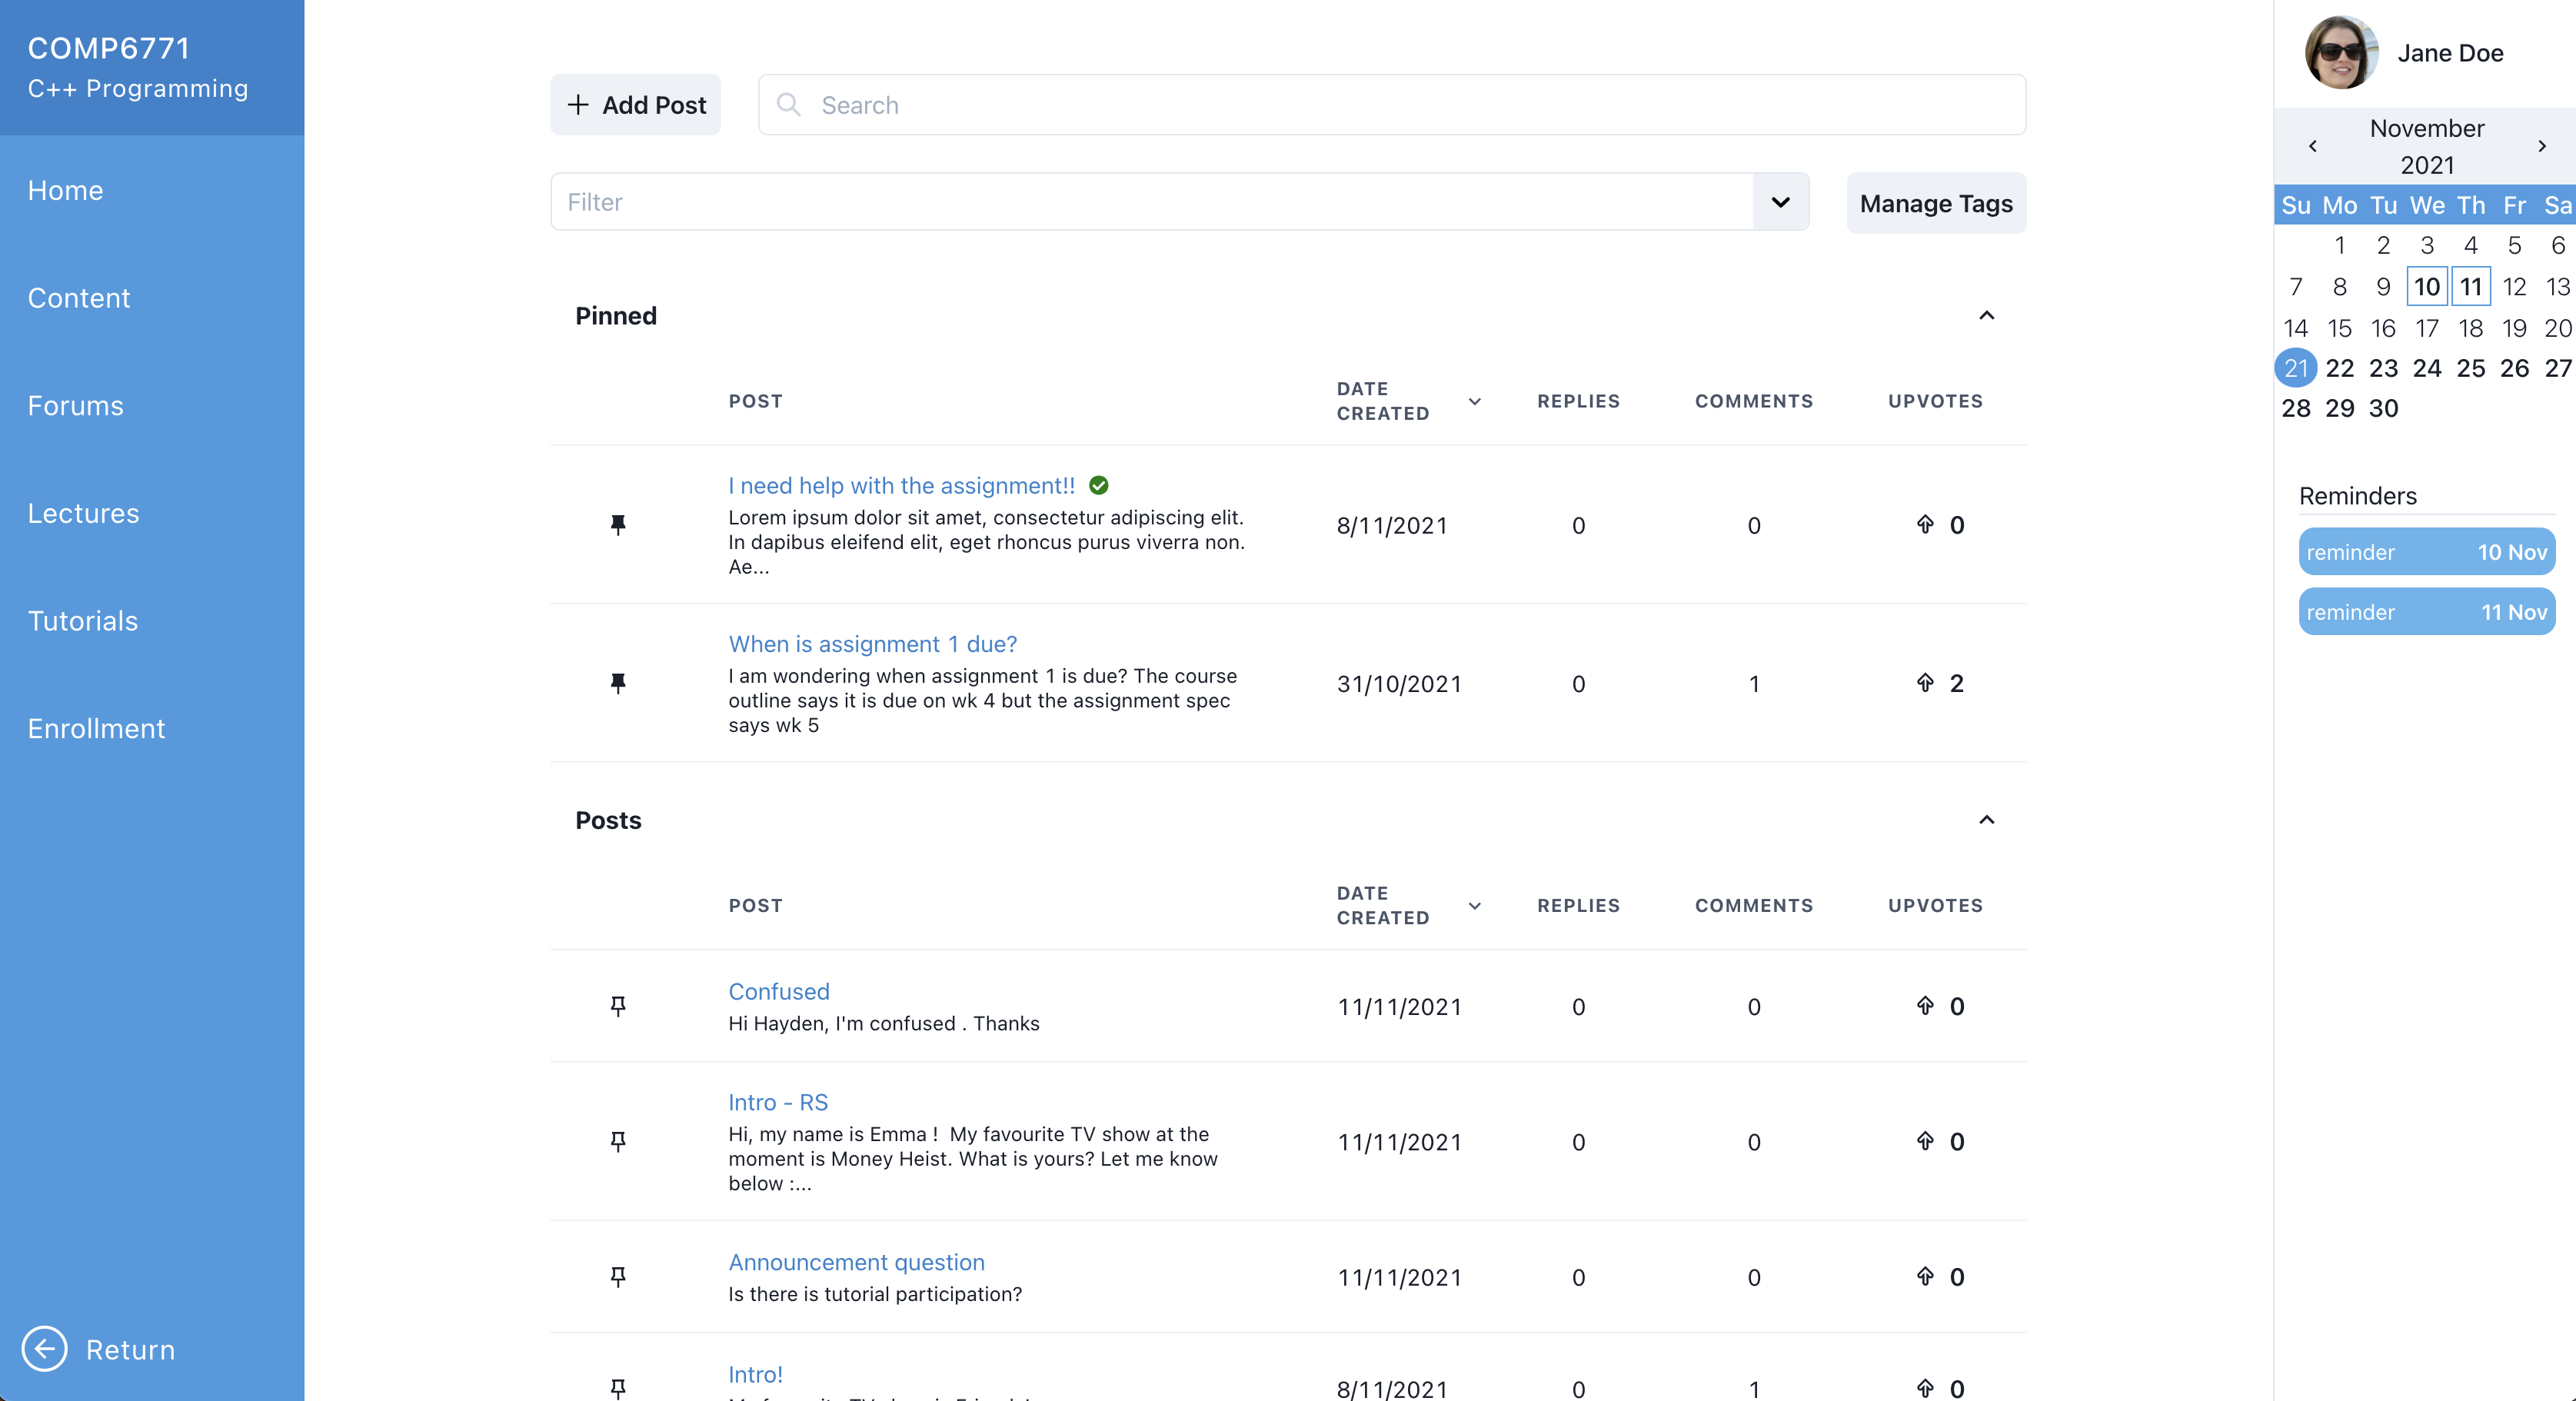
\includegraphics[scale=0.2]{forums-walkthrough-pinned-posts.png}
    \centering
    \caption{Forum overview page for a staff user.}
\end{figure}

\subsubsection{Purpose}
Allows staff to highlight certain forum posts as important.
This assists in bringing these posts to the students' attention.

\subsubsection{What Was Implemented}
Each post in the table has a pin icon next to it.
When a staff user clicks the pin icon for a post in the ``Posts" table, that post will be added to the ``Pinned" posts table.
The pinned post will also continue to show in the regular ``Posts" table but the pin icon will change to a filled pin icon.

Similarly, if a user clicks a filled pin icon, the post will be unpinned and removed from the ``Pinned" post table.

\subsubsection{How It Was Implemented}
When a staff user clicks the button to pin a post, a backend call is made to set the \texttt{isPinned} flag for that post.
This triggers the frontend to re-render so that the post immediately shows in the ``Pinned" table.

Similarly, when a staff user clicks the button to unpin a post, the \texttt{isPinned} flag is set to false and the frontend is re-rendered to reflect the change.

\subsubsection{Considerations}
When a post is pinned, it is still listed in the ``Posts" table, but with a filled pin icon.
By keeping the pinned post in the ``Posts" table, it maintains the chronological order of all the posts.
This is mainly to ensure that no post is missed if a user is simply scrolling through the forum to catch up on new posts.

\subsection{Reply}
Staff users can reply to a post in the responses section of the post's individual page.

\begin{figure}[h!]
    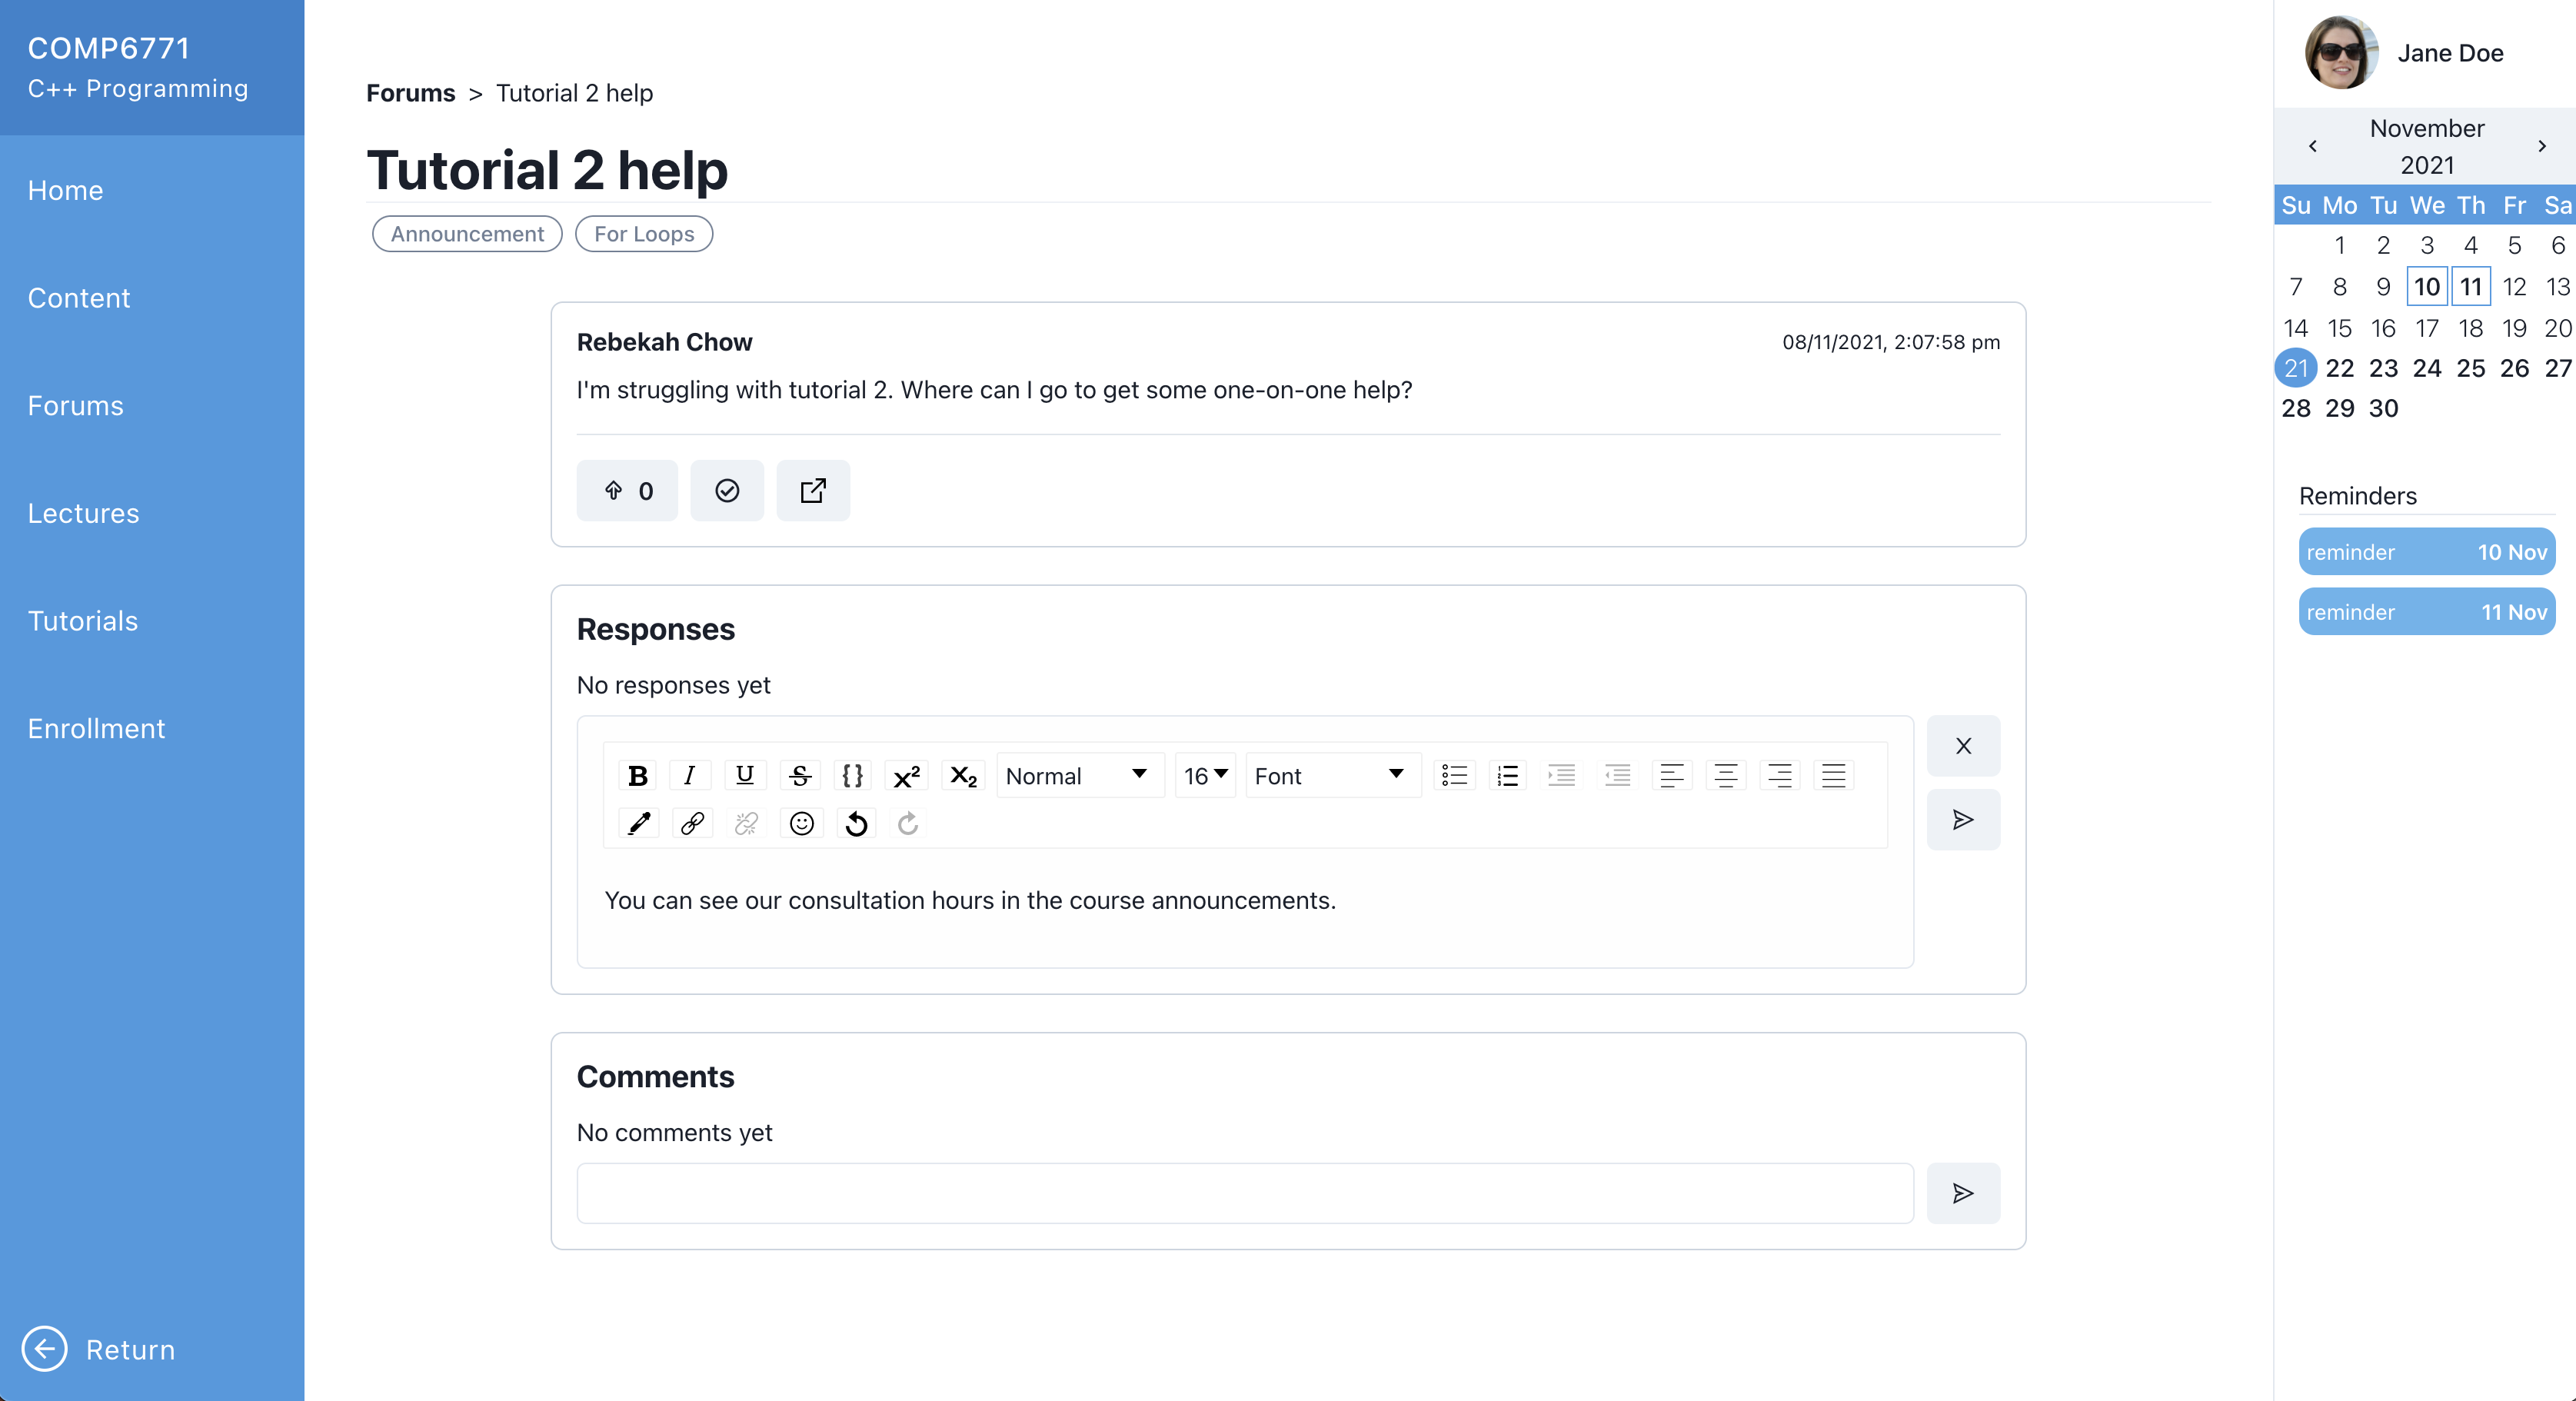
\includegraphics[scale=0.2]{forums-walkthrough-reply.png}
    \centering
    \caption{Leaving a reply on a forum post.}
\end{figure}

\subsubsection{Purpose}
Gives staff users a dedicated area to leave a response to a forum post.

\subsubsection{What Was Implemented}
Similar to comments, staff can click on the input field in the responses section to open the rich-text editor and leave their response.
The rich-text editor allow staff to embed a link to specific resources or course material in their response.

\newpage

Authors of a response will also be able to see buttons for editing and deleting their reply.

\begin{figure}[h!]
    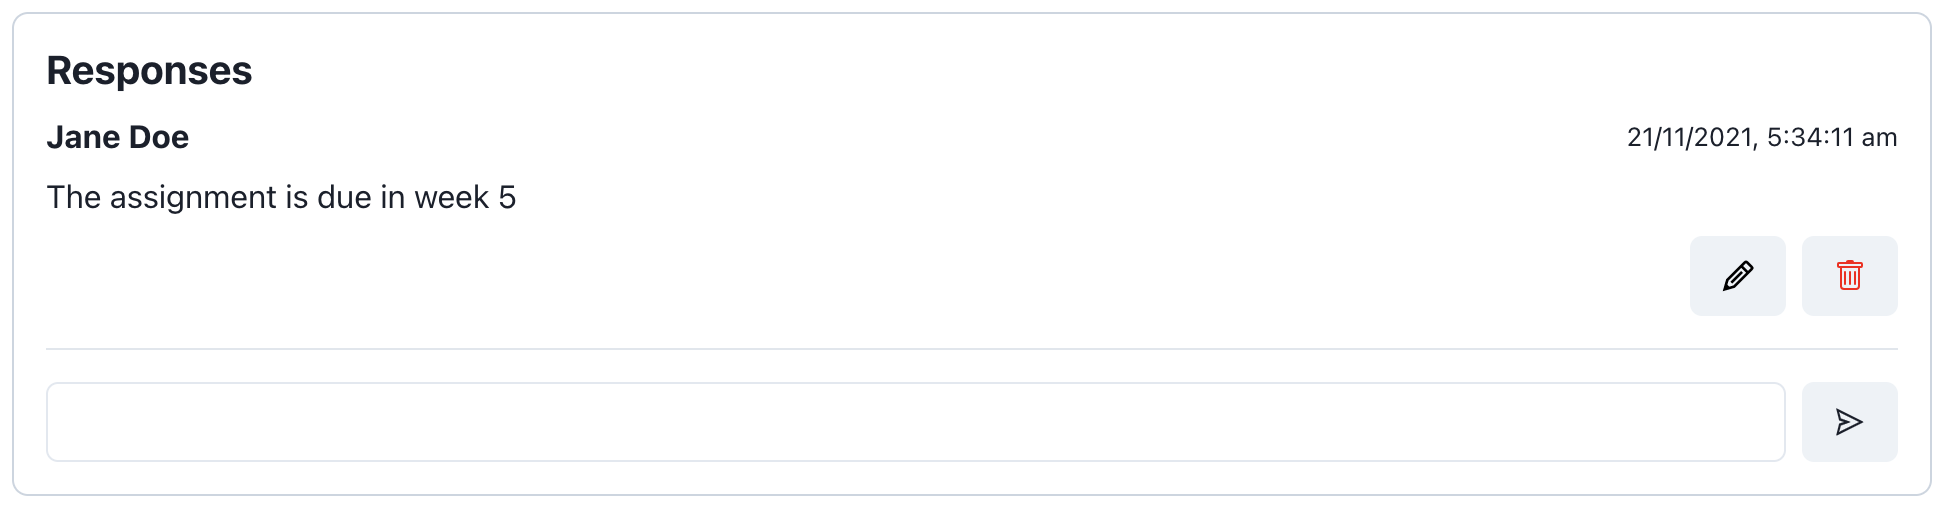
\includegraphics[scale=0.2]{forums-walkthrough-replies-edit-delete.png}
    \centering
    \caption{Reply with edit and delete options}
\end{figure}

For non-staff users, there is no input field visible for the responses section.

\subsubsection{How It Was Implemented}
Similar to posting a comment, clicking on the input field triggers the editor to be initialised.
When the user clicks ``Send", a backend call is made to store the reply in the database, and the frontend is re-rendered to immediately display the response.

Editing and deleting a reply works exactly the same way as editing and deleting posts and comments.

\subsubsection{Considerations}
For the reasons behind separating responses from comments, please see Section 5.6.6.

\newpage

\subsection{Endorsed Posts and Comments}
From the post page, staff users are able to endorse a comment or the whole post by clicking the endorse button.

\begin{figure}[h!]
    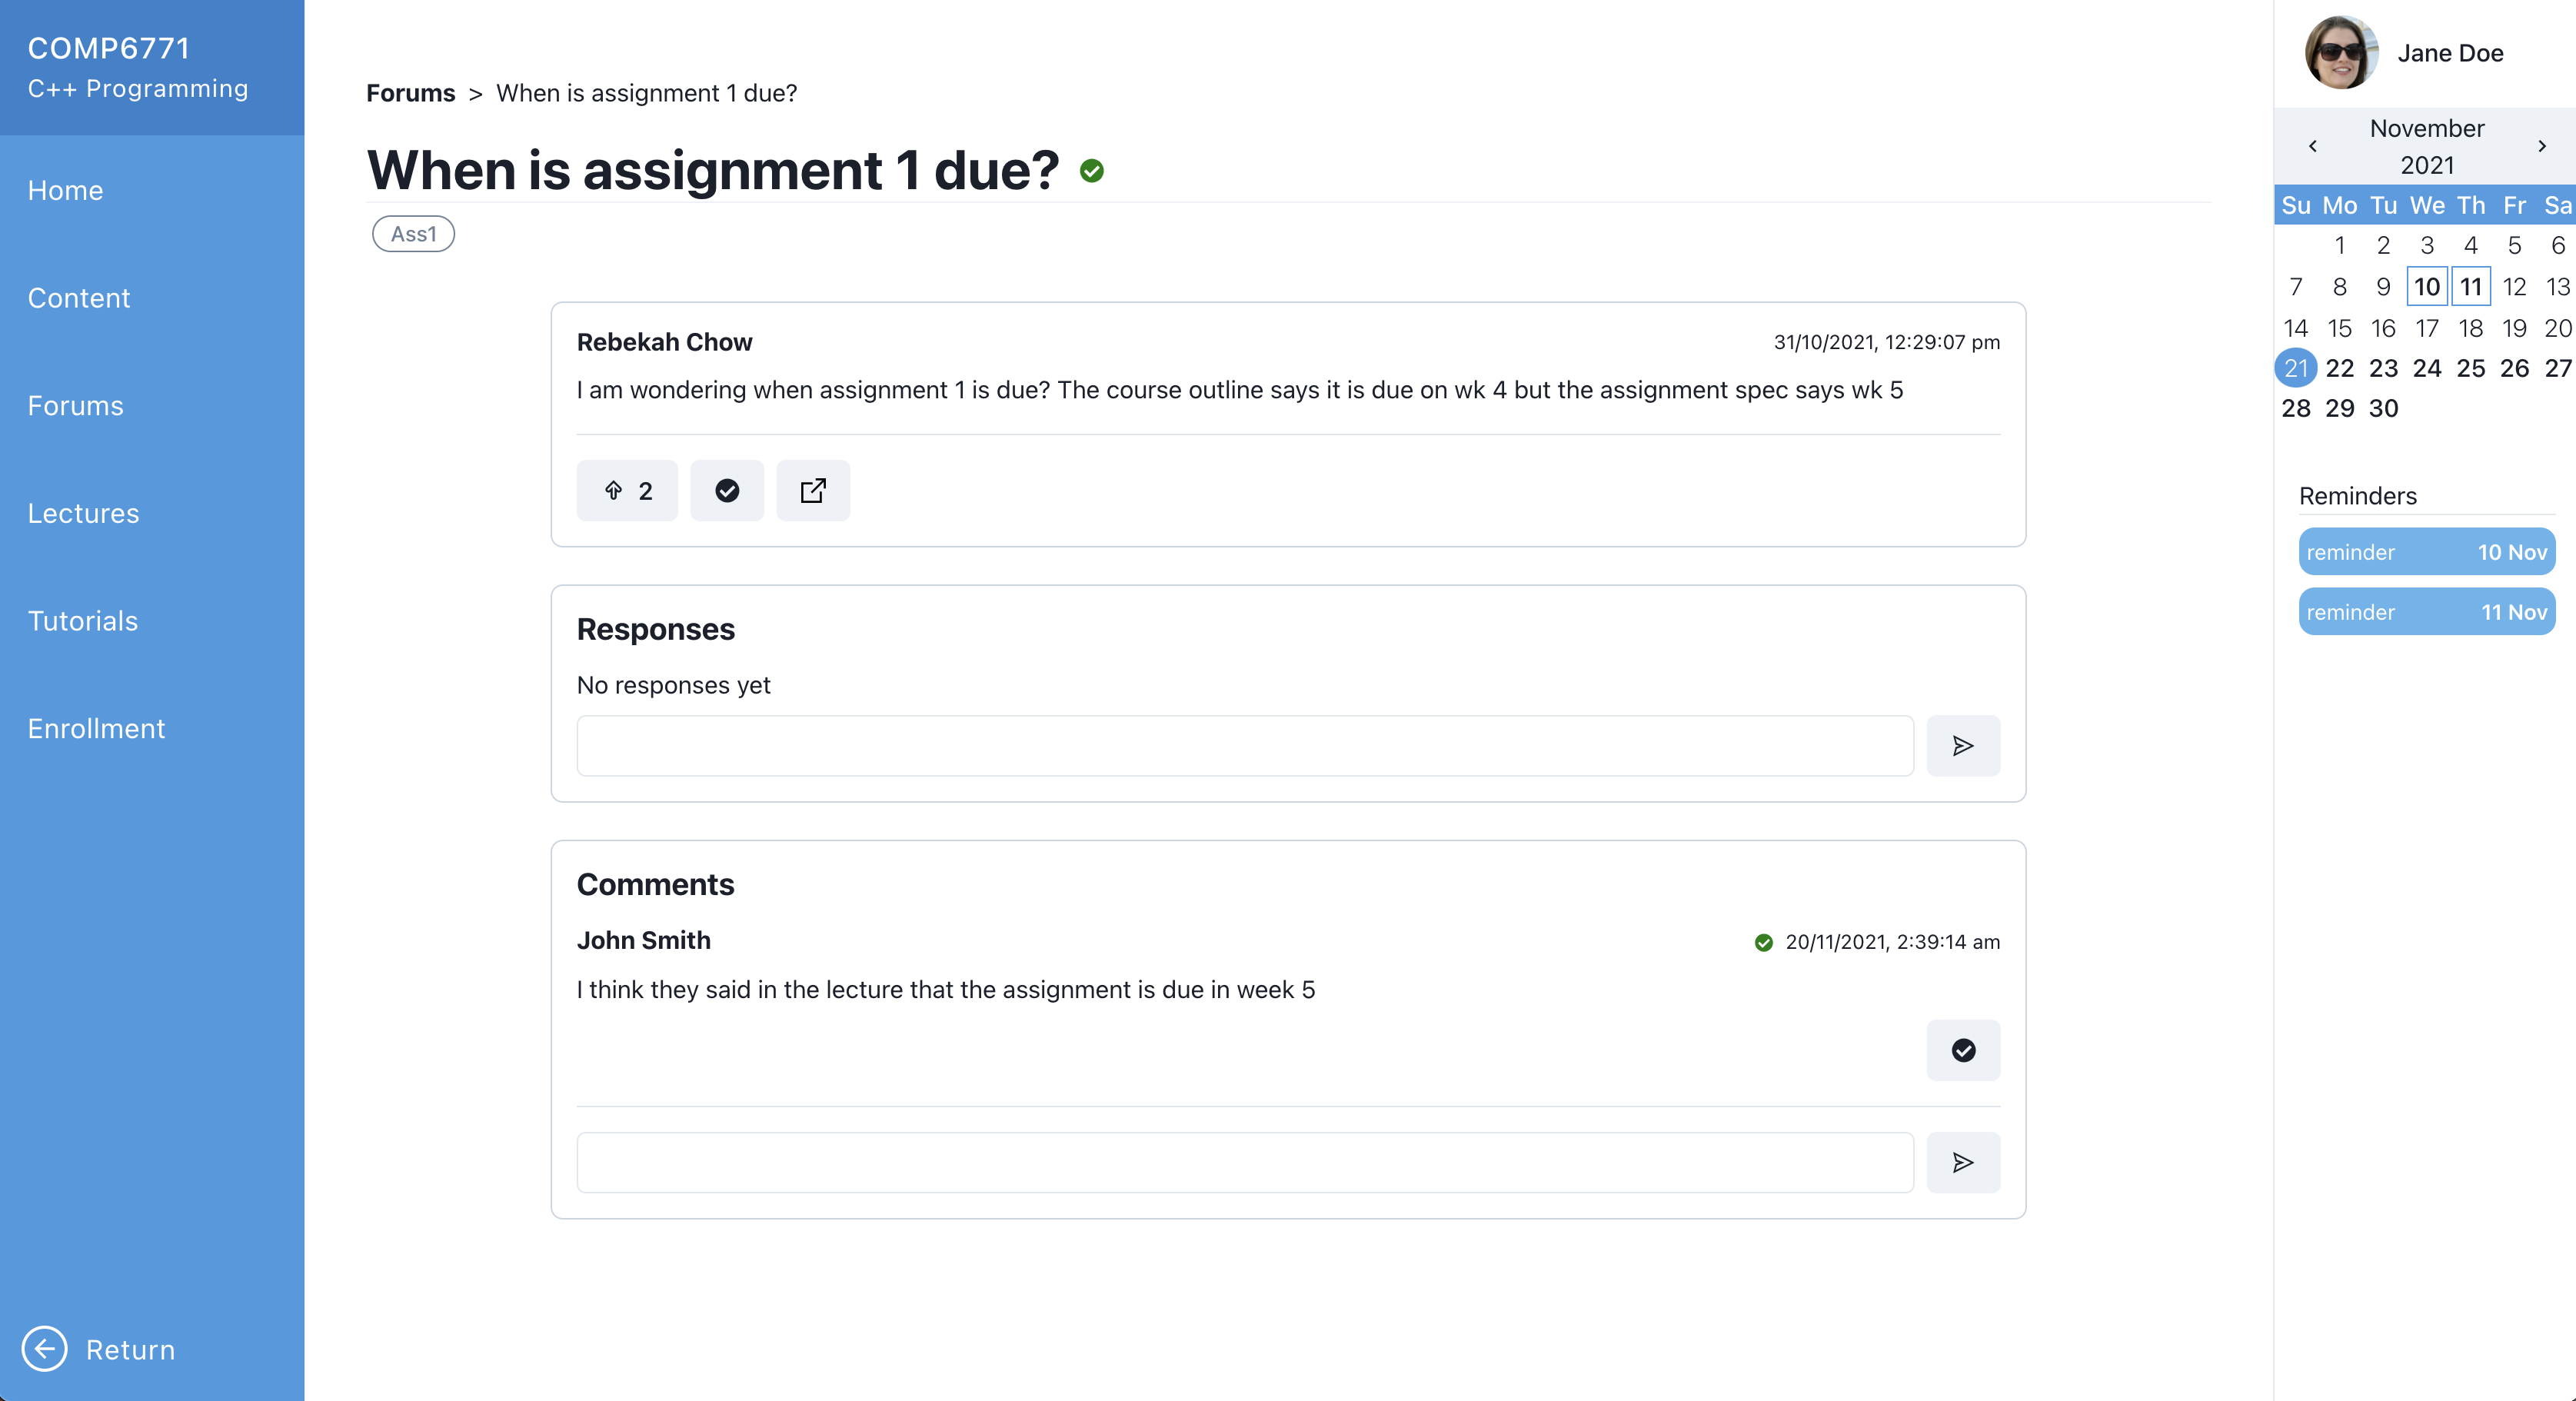
\includegraphics[scale=0.2]{forums-walkthrough-endorse-post-comments.png}
    \centering
    \caption{A post and comment that has been endorsed by staff.}
\end{figure}

\subsubsection{Purpose}
For endorsing a post, it gives staff another way to mark a forum post as important.

For endorsing a comment, it allows staff to verify a student's answer to a question so that other users know that the answer is correct.

\subsubsection{What Was Implemented}
In the post details section of the post page, staff users will see an additional button that has a check mark icon.
Clicking this button will allow staff users to endorse a post, as denoted by the green check mark next to the post title.

Similarly, a staff user can endorse a comment on a post page by clicking the endorse button for that comment.

For more information on the endorse icon for posts and comments, please see Section 5.6.4.

\subsubsection{How It Was Implemented}
When a staff user clicks on the endorse button, it makes a backend call to set the \texttt{isEndorsed} flag to true for the current post.
This triggers the frontend to re-render so that the endorsed icon immediately displays.
The icon on the endorsed button is also filled in to signify that the post has already been endorsed.

When clicked again, the endorsed button will return to the unfilled icon and the endorsement will be removed from the backend.
The endorsed icon on the post or comment will be hidden immediately.

\begin{figure}[h!]
    
\includegraphics[scale=0.5]{forums-walkthrough-endorsed-buttons.png}
    \centering
    \caption{Endorsed buttons that have and haven't been endorsed.}
\end{figure}

\subsubsection{Considerations}
For the reasons behind how the endorsed icon is displayed, please see Section 5.6.4.

It was decided that the ability to endorse responses was not required since they can only be left by staff in the first place and therefore, are already verified.